\chapter{Przebiegi symulacji z zakłóceniem}

Dla dobranych parametrów algorytmu DMC wykonano symulacje dla zmiennego toru zakłócenia mierzalnego. W wyniku symulacji przeprowadzonych podczas doboru parametrów ustalono, że w chwili $k$~=~100 proces ma osiągniętą wartość wyjściową $y(k)$ równą wartości zadanej. Dlatego wszelkie zmiany wartości zakłócenia nastepowały w tej własnie chwili. Za wartość parametru $D_z$ przyjęto $D_z$~=~\num{201}, będące długością uzyskanej odpowiedzi skokowej toru zakłócenie-wyjście.


\section{Dla skokowej zmiany zakłócenia}

Zasymulowano przebiegi procesu dla zmiany wartości zakłócenia mierzalnego z wartości 0 na wartość 1 w chwili odpowiadającej 100-nej próbce symulacji. Symulacje uruchomiono w w dwóch trybach pracy algorytmu DMC.

\subsection{Bez uwzględniania zakłóceń}

W trybie pracy algorytmu bez uwzględniania zakłóceń otrzymano wskaźnik jakości $e$~=~\num{12.8721}. Przebieg przedstawiono na rysunku \ref{5przebieg}

\begin{figure}
	
	\centering
	\caption{ Przebieg symulacji algorytmu DMC dla skoku zakłócenia bez uwzględniania zakłóceń }
	% This file was created by matlab2tikz.
%
%The latest updates can be retrieved from
%  http://www.mathworks.com/matlabcentral/fileexchange/22022-matlab2tikz-matlab2tikz
%where you can also make suggestions and rate matlab2tikz.
%
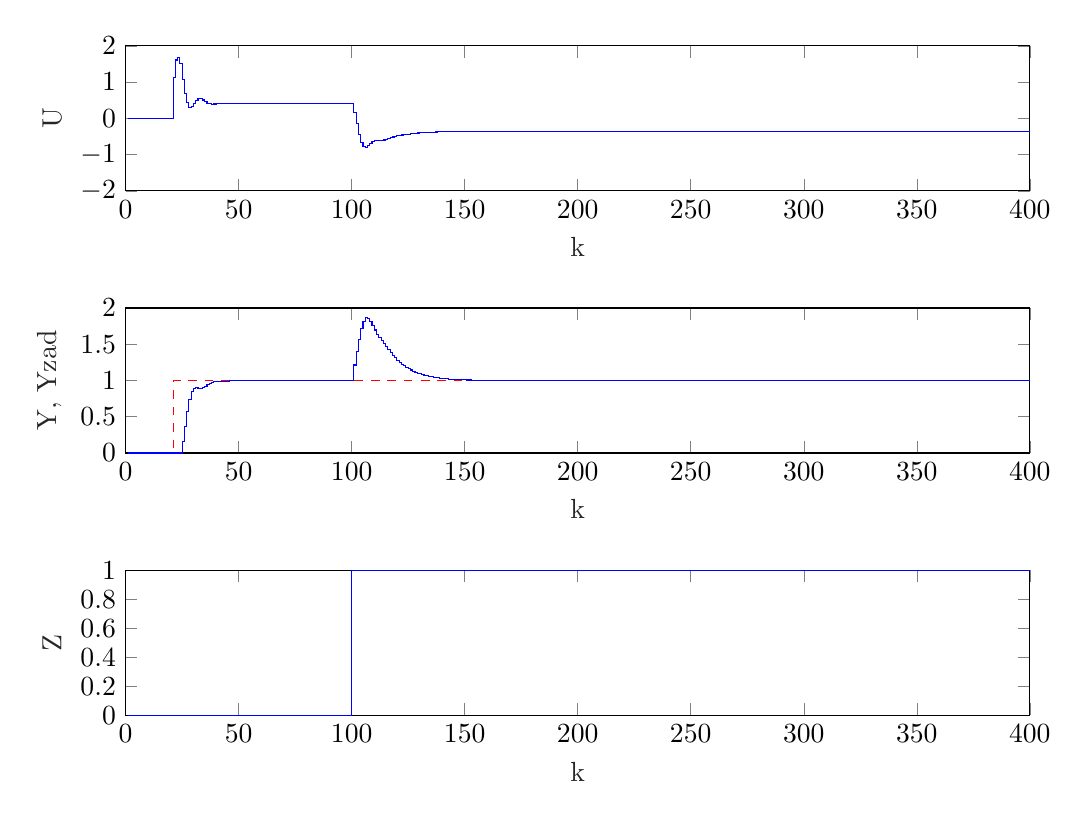
\begin{tikzpicture}

\begin{axis}[%
width=4.521in,
height=0.725in,
at={(0.758in,3.322in)},
scale only axis,
xmin=0,
xmax=400,
xlabel style={font=\color{white!15!black}},
xlabel={k},
ymin=-2,
ymax=2,
ylabel style={font=\color{white!15!black}},
ylabel={U},
axis background/.style={fill=white}
]
\addplot[const plot, color=blue, forget plot] table[row sep=crcr] {%
1	0\\
2	0\\
3	0\\
4	0\\
5	0\\
6	0\\
7	0\\
8	0\\
9	0\\
10	0\\
11	0\\
12	0\\
13	0\\
14	0\\
15	0\\
16	0\\
17	0\\
18	0\\
19	0\\
20	0\\
21	1.13124041331753\\
22	1.60739620208848\\
23	1.67029772812697\\
24	1.5088290696095\\
25	1.08258009935487\\
26	0.684037120257817\\
27	0.424015380122655\\
28	0.310055013493176\\
29	0.329911659559614\\
30	0.412055543717462\\
31	0.49284813281035\\
32	0.53826796688865\\
33	0.537912993315766\\
34	0.504308140292631\\
35	0.45877281065022\\
36	0.419410565589577\\
37	0.396275443971251\\
38	0.390196587205243\\
39	0.395737940223536\\
40	0.405530115035693\\
41	0.413556147410279\\
42	0.416831988264799\\
43	0.415363749413303\\
44	0.41100616794113\\
45	0.406084453780792\\
46	0.402349250225408\\
47	0.40052789855623\\
48	0.400422166673599\\
49	0.401311205757422\\
50	0.402400609633999\\
51	0.403135629315426\\
52	0.403312371317209\\
53	0.403020350347085\\
54	0.402499132197402\\
55	0.401993011482922\\
56	0.401657765772953\\
57	0.40153450897489\\
58	0.401575545994931\\
59	0.40169360029823\\
60	0.40180770201165\\
61	0.401870068243431\\
62	0.401871046600647\\
63	0.40182832958733\\
64	0.401770153994924\\
65	0.401720848379131\\
66	0.401693163682481\\
67	0.401687705971358\\
68	0.401697066358232\\
69	0.40171140175517\\
70	0.401722879568028\\
71	0.401727766843836\\
72	0.401726257840868\\
73	0.401720930851284\\
74	0.401714902237765\\
75	0.401710465406525\\
76	0.401708535593691\\
77	0.401708807856827\\
78	0.40171030785626\\
79	0.401711988442695\\
80	0.401713135670161\\
81	0.401713504677854\\
82	0.401713234372025\\
83	0.401712653194794\\
84	0.401712087119452\\
85	0.401711739451988\\
86	0.401711660141687\\
87	0.401711782952107\\
88	0.401711991877851\\
89	0.401712181631659\\
90	0.401712292121399\\
91	0.40171231376668\\
92	0.401712272378503\\
93	0.401712206636815\\
94	0.401712149141236\\
95	0.401712116674031\\
96	0.401712109863984\\
97	0.401712118919425\\
98	0.401712131093258\\
99	0.401712136499113\\
100	0.401712130744792\\
101	0.160475096441706\\
102	-0.155227652291736\\
103	-0.448906935162451\\
104	-0.675180934884802\\
105	-0.78514450680548\\
106	-0.79775571849983\\
107	-0.753479043993001\\
108	-0.689847674993846\\
109	-0.637572458106992\\
110	-0.60866408148127\\
111	-0.600213951069078\\
112	-0.602384210919803\\
113	-0.604222364160676\\
114	-0.59867579347581\\
115	-0.58402974603963\\
116	-0.562622631557903\\
117	-0.538674597540242\\
118	-0.51610906900605\\
119	-0.497249899541557\\
120	-0.482588525395148\\
121	-0.471277979545612\\
122	-0.461929868899412\\
123	-0.453312817222692\\
124	-0.444729098373045\\
125	-0.436055102826766\\
126	-0.427554394567246\\
127	-0.419616042667845\\
128	-0.412543152405001\\
129	-0.406451057971032\\
130	-0.401272705400855\\
131	-0.396830228730424\\
132	-0.392922210073268\\
133	-0.389388897915761\\
134	-0.386139535133235\\
135	-0.383145628724309\\
136	-0.380415088453847\\
137	-0.377963690683369\\
138	-0.375795257508175\\
139	-0.373894558006137\\
140	-0.372230792074506\\
141	-0.370766415881674\\
142	-0.369466031313605\\
143	-0.368301977789564\\
144	-0.367255713647973\\
145	-0.366315960261145\\
146	-0.365475418692711\\
147	-0.364727733684291\\
148	-0.364065678970316\\
149	-0.36348073631126\\
150	-0.36296366960275\\
151	-0.362505480070081\\
152	-0.362098217483783\\
153	-0.361735371222798\\
154	-0.361411823754341\\
155	-0.3611235190477\\
156	-0.360867049758833\\
157	-0.360639324402922\\
158	-0.360437389310999\\
159	-0.360258397775652\\
160	-0.360099669231182\\
161	-0.359958770759214\\
162	-0.359833571242472\\
163	-0.359722248009516\\
164	-0.359623251776699\\
165	-0.359535249880909\\
166	-0.359457069328759\\
167	-0.359387654155824\\
168	-0.35932604172824\\
169	-0.359271354597499\\
170	-0.359222800617021\\
171	-0.359179674175229\\
172	-0.359141354061853\\
173	-0.359107296767002\\
174	-0.359077026487803\\
175	-0.359050124176978\\
176	-0.359026217745981\\
177	-0.359004974587762\\
178	-0.358986096528489\\
179	-0.358969316584276\\
180	-0.358954396641799\\
181	-0.358941125322923\\
182	-0.358929315637136\\
183	-0.358918802373127\\
184	-0.358909439404964\\
185	-0.358901097153389\\
186	-0.358893660384703\\
187	-0.358887026416182\\
188	-0.358881103691134\\
189	-0.358875810625549\\
190	-0.358871074618793\\
191	-0.358866831148168\\
192	-0.35886302290861\\
193	-0.358859598994399\\
194	-0.358856514139238\\
195	-0.358853728033592\\
196	-0.358851204729446\\
197	-0.358848912130455\\
198	-0.35884682155578\\
199	-0.358844907361762\\
200	-0.358843146606656\\
201	-0.358841518747936\\
202	-0.358840005366544\\
203	-0.35883858991619\\
204	-0.358837257497522\\
205	-0.358835994657009\\
206	-0.358834789209388\\
207	-0.358833630081451\\
208	-0.358832507174231\\
209	-0.358831411240577\\
210	-0.358830333775503\\
211	-0.358829266917378\\
212	-0.358828203358605\\
213	-0.358827136264891\\
214	-0.358826059202421\\
215	-0.358824966072251\\
216	-0.358823851051213\\
217	-0.358822728285484\\
218	-0.358821693478298\\
219	-0.358821015098431\\
220	-0.358820875339334\\
221	-0.358821293019439\\
222	-0.358822128766484\\
223	-0.358825934128604\\
224	-0.3588318356639\\
225	-0.358837974762601\\
226	-0.358842794246422\\
227	-0.358844646568678\\
228	-0.358843353236184\\
229	-0.358839951032459\\
230	-0.358835913252054\\
231	-0.358832687694338\\
232	-0.358831077701203\\
233	-0.35883108240932\\
234	-0.358832133496212\\
235	-0.358833436411298\\
236	-0.358834333968723\\
237	-0.358834519274962\\
238	-0.3588340469545\\
239	-0.35883321021982\\
240	-0.358832361383505\\
241	-0.358831761478428\\
242	-0.358831509996203\\
243	-0.358831555761273\\
244	-0.358831760983533\\
245	-0.358831978360463\\
246	-0.358832107880802\\
247	-0.358832118454955\\
248	-0.35883203722303\\
249	-0.358831920648622\\
250	-0.358831823992828\\
251	-0.358831781056996\\
252	-0.358831798447756\\
253	-0.358831861827572\\
254	-0.35883194794111\\
255	-0.35883203606591\\
256	-0.358832114817531\\
257	-0.358832183298672\\
258	-0.35883224802088\\
259	-0.358832318131025\\
260	-0.358832401269863\\
261	-0.358832501385443\\
262	-0.358832618659351\\
263	-0.358832750867393\\
264	-0.358832895190927\\
265	-0.358833049657404\\
266	-0.358833213801846\\
267	-0.358833388566992\\
268	-0.35883357573602\\
269	-0.358833777265692\\
270	-0.358833994800368\\
271	-0.358834229485519\\
272	-0.358834482048472\\
273	-0.358834753026398\\
274	-0.358835043008092\\
275	-0.358835352796637\\
276	-0.358835683461094\\
277	-0.358836036297332\\
278	-0.358836412744908\\
279	-0.358836814307077\\
280	-0.358837242503841\\
281	-0.358837698865518\\
282	-0.358838184956908\\
283	-0.358838702414358\\
284	-0.358839252979488\\
285	-0.358839838520277\\
286	-0.35884046103822\\
287	-0.358841122665951\\
288	-0.35884182566185\\
289	-0.358842572407132\\
290	-0.358843365408233\\
291	-0.358844207304499\\
292	-0.358845100879409\\
293	-0.358846049072988\\
294	-0.358847054993645\\
295	-0.358848121928632\\
296	-0.358849253353312\\
297	-0.358850448728916\\
298	-0.358851686629394\\
299	-0.358852890304445\\
300	-0.358853952342117\\
301	-0.358854773000612\\
302	-0.358855293127964\\
303	-0.358854915809109\\
304	-0.35885329713519\\
305	-0.358850527938882\\
306	-0.358847020756174\\
307	-0.358843493013091\\
308	-0.358840619543226\\
309	-0.358838778213475\\
310	-0.358837990170322\\
311	-0.358837965320753\\
312	-0.358838274709084\\
313	-0.358838537619141\\
314	-0.35883853719284\\
315	-0.358838250302434\\
316	-0.358837796528938\\
317	-0.358837347454683\\
318	-0.358837043738426\\
319	-0.358836947710511\\
320	-0.358837039564531\\
321	-0.358837246046302\\
322	-0.358837480907776\\
323	-0.358837678502607\\
324	-0.358837809951923\\
325	-0.358837881052953\\
326	-0.358837918307937\\
327	-0.358837951907429\\
328	-0.358838002902951\\
329	-0.358838077983424\\
330	-0.358838171347743\\
331	-0.358838270687385\\
332	-0.358838363720884\\
333	-0.358838442662189\\
334	-0.358838505622989\\
335	-0.358838555415793\\
336	-0.358838597040159\\
337	-0.358838635206054\\
338	-0.358838672791766\\
339	-0.358838710493075\\
340	-0.358838747395235\\
341	-0.358838781947366\\
342	-0.358838812843545\\
343	-0.35883883951515\\
344	-0.358838862182026\\
345	-0.358838881591033\\
346	-0.358838898643263\\
347	-0.358838914084773\\
348	-0.358838928353443\\
349	-0.358838941585698\\
350	-0.358838953726617\\
351	-0.358838964667985\\
352	-0.358838974354196\\
353	-0.358838982828251\\
354	-0.358838990221657\\
355	-0.358838996711435\\
356	-0.358839002471644\\
357	-0.358839007639426\\
358	-0.358839012303392\\
359	-0.358839016511201\\
360	-0.358839020287173\\
361	-0.358839023650246\\
362	-0.358839026625733\\
363	-0.358839029248902\\
364	-0.358839031562056\\
365	-0.3588390336086\\
366	-0.358839035427465\\
367	-0.358839037049961\\
368	-0.358839038499478\\
369	-0.35883903979328\\
370	-0.358839040945092\\
371	-0.35883904196735\\
372	-0.358839042872473\\
373	-0.358839043673107\\
374	-0.358839044381676\\
375	-0.358839045009694\\
376	-0.358839045567239\\
377	-0.358839046062758\\
378	-0.358839046503215\\
379	-0.358839046894428\\
380	-0.35883904724145\\
381	-0.358839047548863\\
382	-0.358839047820932\\
383	-0.358839048061637\\
384	-0.358839048274632\\
385	-0.358839048463196\\
386	-0.358839048630203\\
387	-0.358839048778141\\
388	-0.358839048909163\\
389	-0.358839049025149\\
390	-0.358839049127767\\
391	-0.358839049218526\\
392	-0.358839049298792\\
393	-0.358839049369808\\
394	-0.358839049432694\\
395	-0.358839049488454\\
396	-0.358839049537981\\
397	-0.358839049582066\\
398	-0.358839049621419\\
399	-0.358839049656677\\
400	-0.358839049688416\\
};
\end{axis}

\begin{axis}[%
width=4.521in,
height=0.725in,
at={(0.758in,2.011in)},
scale only axis,
xmin=0,
xmax=400,
xlabel style={font=\color{white!15!black}},
xlabel={k},
ymin=0,
ymax=2,
ylabel style={font=\color{white!15!black}},
ylabel={Y, Yzad},
axis background/.style={fill=white}
]
\addplot[const plot, color=red, dashed, forget plot] table[row sep=crcr] {%
1	0\\
2	0\\
3	0\\
4	0\\
5	0\\
6	0\\
7	0\\
8	0\\
9	0\\
10	0\\
11	0\\
12	0\\
13	0\\
14	0\\
15	0\\
16	0\\
17	0\\
18	0\\
19	0\\
20	0\\
21	1\\
22	1\\
23	1\\
24	1\\
25	1\\
26	1\\
27	1\\
28	1\\
29	1\\
30	1\\
31	1\\
32	1\\
33	1\\
34	1\\
35	1\\
36	1\\
37	1\\
38	1\\
39	1\\
40	1\\
41	1\\
42	1\\
43	1\\
44	1\\
45	1\\
46	1\\
47	1\\
48	1\\
49	1\\
50	1\\
51	1\\
52	1\\
53	1\\
54	1\\
55	1\\
56	1\\
57	1\\
58	1\\
59	1\\
60	1\\
61	1\\
62	1\\
63	1\\
64	1\\
65	1\\
66	1\\
67	1\\
68	1\\
69	1\\
70	1\\
71	1\\
72	1\\
73	1\\
74	1\\
75	1\\
76	1\\
77	1\\
78	1\\
79	1\\
80	1\\
81	1\\
82	1\\
83	1\\
84	1\\
85	1\\
86	1\\
87	1\\
88	1\\
89	1\\
90	1\\
91	1\\
92	1\\
93	1\\
94	1\\
95	1\\
96	1\\
97	1\\
98	1\\
99	1\\
100	1\\
101	1\\
102	1\\
103	1\\
104	1\\
105	1\\
106	1\\
107	1\\
108	1\\
109	1\\
110	1\\
111	1\\
112	1\\
113	1\\
114	1\\
115	1\\
116	1\\
117	1\\
118	1\\
119	1\\
120	1\\
121	1\\
122	1\\
123	1\\
124	1\\
125	1\\
126	1\\
127	1\\
128	1\\
129	1\\
130	1\\
131	1\\
132	1\\
133	1\\
134	1\\
135	1\\
136	1\\
137	1\\
138	1\\
139	1\\
140	1\\
141	1\\
142	1\\
143	1\\
144	1\\
145	1\\
146	1\\
147	1\\
148	1\\
149	1\\
150	1\\
151	1\\
152	1\\
153	1\\
154	1\\
155	1\\
156	1\\
157	1\\
158	1\\
159	1\\
160	1\\
161	1\\
162	1\\
163	1\\
164	1\\
165	1\\
166	1\\
167	1\\
168	1\\
169	1\\
170	1\\
171	1\\
172	1\\
173	1\\
174	1\\
175	1\\
176	1\\
177	1\\
178	1\\
179	1\\
180	1\\
181	1\\
182	1\\
183	1\\
184	1\\
185	1\\
186	1\\
187	1\\
188	1\\
189	1\\
190	1\\
191	1\\
192	1\\
193	1\\
194	1\\
195	1\\
196	1\\
197	1\\
198	1\\
199	1\\
200	1\\
201	1\\
202	1\\
203	1\\
204	1\\
205	1\\
206	1\\
207	1\\
208	1\\
209	1\\
210	1\\
211	1\\
212	1\\
213	1\\
214	1\\
215	1\\
216	1\\
217	1\\
218	1\\
219	1\\
220	1\\
221	1\\
222	1\\
223	1\\
224	1\\
225	1\\
226	1\\
227	1\\
228	1\\
229	1\\
230	1\\
231	1\\
232	1\\
233	1\\
234	1\\
235	1\\
236	1\\
237	1\\
238	1\\
239	1\\
240	1\\
241	1\\
242	1\\
243	1\\
244	1\\
245	1\\
246	1\\
247	1\\
248	1\\
249	1\\
250	1\\
251	1\\
252	1\\
253	1\\
254	1\\
255	1\\
256	1\\
257	1\\
258	1\\
259	1\\
260	1\\
261	1\\
262	1\\
263	1\\
264	1\\
265	1\\
266	1\\
267	1\\
268	1\\
269	1\\
270	1\\
271	1\\
272	1\\
273	1\\
274	1\\
275	1\\
276	1\\
277	1\\
278	1\\
279	1\\
280	1\\
281	1\\
282	1\\
283	1\\
284	1\\
285	1\\
286	1\\
287	1\\
288	1\\
289	1\\
290	1\\
291	1\\
292	1\\
293	1\\
294	1\\
295	1\\
296	1\\
297	1\\
298	1\\
299	1\\
300	1\\
301	1\\
302	1\\
303	1\\
304	1\\
305	1\\
306	1\\
307	1\\
308	1\\
309	1\\
310	1\\
311	1\\
312	1\\
313	1\\
314	1\\
315	1\\
316	1\\
317	1\\
318	1\\
319	1\\
320	1\\
321	1\\
322	1\\
323	1\\
324	1\\
325	1\\
326	1\\
327	1\\
328	1\\
329	1\\
330	1\\
331	1\\
332	1\\
333	1\\
334	1\\
335	1\\
336	1\\
337	1\\
338	1\\
339	1\\
340	1\\
341	1\\
342	1\\
343	1\\
344	1\\
345	1\\
346	1\\
347	1\\
348	1\\
349	1\\
350	1\\
351	1\\
352	1\\
353	1\\
354	1\\
355	1\\
356	1\\
357	1\\
358	1\\
359	1\\
360	1\\
361	1\\
362	1\\
363	1\\
364	1\\
365	1\\
366	1\\
367	1\\
368	1\\
369	1\\
370	1\\
371	1\\
372	1\\
373	1\\
374	1\\
375	1\\
376	1\\
377	1\\
378	1\\
379	1\\
380	1\\
381	1\\
382	1\\
383	1\\
384	1\\
385	1\\
386	1\\
387	1\\
388	1\\
389	1\\
390	1\\
391	1\\
392	1\\
393	1\\
394	1\\
395	1\\
396	1\\
397	1\\
398	1\\
399	1\\
400	1\\
};
\addplot[const plot, color=blue, forget plot] table[row sep=crcr] {%
1	0\\
2	0\\
3	0\\
4	0\\
5	0\\
6	0\\
7	0\\
8	0\\
9	0\\
10	0\\
11	0\\
12	0\\
13	0\\
14	0\\
15	0\\
16	0\\
17	0\\
18	0\\
19	0\\
20	0\\
21	0\\
22	0\\
23	0\\
24	0\\
25	0.152830579839198\\
26	0.361723685979986\\
27	0.567813252929803\\
28	0.740934525440941\\
29	0.847095360437015\\
30	0.893658115143514\\
31	0.90255973864811\\
32	0.895570671873684\\
33	0.89163036498361\\
34	0.898990405246294\\
35	0.91685828271975\\
36	0.939887677878803\\
37	0.961615803129477\\
38	0.977621370527924\\
39	0.986602460199098\\
40	0.989773437013205\\
41	0.989641380644215\\
42	0.988689847199495\\
43	0.988533654813312\\
44	0.989704626042417\\
45	0.991892848316057\\
46	0.994401945347177\\
47	0.996573965969035\\
48	0.998037076898529\\
49	0.998753666950623\\
50	0.998924656597726\\
51	0.998838350857697\\
52	0.998740665168325\\
53	0.998766808279368\\
54	0.998937329483177\\
55	0.999196697549384\\
56	0.999464818354491\\
57	0.999678006297738\\
58	0.999808372281484\\
59	0.999862529279366\\
60	0.999867769339971\\
61	0.999855454910885\\
62	0.999848800913543\\
63	0.999857968169211\\
64	0.999881621834702\\
65	0.999912037309881\\
66	0.999940598025195\\
67	0.999961538784302\\
68	0.999973216807206\\
69	0.999977361349574\\
70	0.999977327623101\\
71	0.999976368399375\\
72	0.999976556980123\\
73	0.999978522354457\\
74	0.999981799158156\\
75	0.999985440953475\\
76	0.999988577040411\\
77	0.999990730653257\\
78	0.99999187053213\\
79	0.999992275801492\\
80	0.999992333120867\\
81	0.99999236613075\\
82	0.999992548519416\\
83	0.999992902381439\\
84	0.999993351510946\\
85	0.999993790164412\\
86	0.999994136571704\\
87	0.999994357305398\\
88	0.999994464385011\\
89	0.999994496292151\\
90	0.999994495860299\\
91	0.999994494377281\\
92	0.999994505516522\\
93	0.999994527765157\\
94	0.999994551375948\\
95	0.999994565659013\\
96	0.999994563834085\\
97	0.999994544575335\\
98	0.999994510910527\\
99	0.999994467862375\\
100	0.999994420170427\\
101	1.2132443709093\\
102	1.40256084618896\\
103	1.57062529004848\\
104	1.71981897655279\\
105	1.81966547754278\\
106	1.8637451689591\\
107	1.85891332261007\\
108	1.81768975773037\\
109	1.75843906801614\\
110	1.69589547195372\\
111	1.63846178402568\\
112	1.58895517062073\\
113	1.54583756580882\\
114	1.50598360490527\\
115	1.46678747206765\\
116	1.42707577036301\\
117	1.38718490980657\\
118	1.348356338578\\
119	1.31196975862356\\
120	1.27899098703012\\
121	1.24974270962403\\
122	1.22398166164581\\
123	1.20114740315328\\
124	1.18062887669876\\
125	1.16194960620771\\
126	1.14483502411862\\
127	1.12918163079815\\
128	1.11497678959748\\
129	1.10221726102389\\
130	1.09085728373044\\
131	1.08079471426123\\
132	1.0718863975045\\
133	1.06397638178213\\
134	1.05692181090698\\
135	1.05060768338761\\
136	1.04494896849931\\
137	1.03988374687288\\
138	1.03536298560428\\
139	1.03134173631942\\
140	1.02777426846738\\
141	1.02461329044278\\
142	1.02181186353991\\
143	1.0193261473911\\
144	1.01711750486686\\
145	1.0151532817726\\
146	1.01340632646465\\
147	1.0118537649348\\
148	1.01047564216144\\
149	1.00925387584049\\
150	1.00817169980629\\
151	1.00721353843996\\
152	1.00636512480624\\
153	1.00561366197075\\
154	1.00494789154458\\
155	1.00435802371356\\
156	1.00383555634089\\
157	1.00337304648067\\
158	1.00296389650735\\
159	1.00260219303927\\
160	1.00228260718037\\
161	1.00200034231544\\
162	1.00175110629278\\
163	1.00153108707046\\
164	1.00133691972357\\
165	1.00116564248423\\
166	1.00101464629868\\
167	1.00088162484479\\
168	1.00076453077395\\
169	1.00066154091097\\
170	1.0005710300742\\
171	1.00049155122427\\
172	1.0004218191359\\
173	1.00036069538563\\
174	1.00030717354356\\
175	1.00026036447386\\
176	1.00021948225239\\
177	1.00018383133766\\
178	1.00015279541886\\
179	1.00012582802116\\
180	1.00010244465389\\
181	1.0000822161376\\
182	1.00006476274668\\
183	1.00004974890549\\
184	1.00003687830577\\
185	1.00002588941804\\
186	1.00001655142211\\
187	1.00000866058526\\
188	1.00000203708943\\
189	0.99999652227481\\
190	0.999991976242589\\
191	0.999988275752588\\
192	0.999985312358441\\
193	0.99998299073861\\
194	0.999981227197324\\
195	0.999979948321016\\
196	0.999979089781165\\
197	0.999978595274731\\
198	0.999978415591127\\
199	0.999978507792205\\
200	0.999978834490695\\
201	0.999979363213196\\
202	0.999980065835839\\
203	0.999980918083193\\
204	0.999981899083283\\
205	0.999982990973088\\
206	0.999984178549808\\
207	0.999985448963479\\
208	0.999986791446622\\
209	0.999988197076721\\
210	0.999989658567598\\
211	0.999991170086115\\
212	0.999992727091156\\
213	0.999994326192311\\
214	0.999995965026082\\
215	0.999997642147782\\
216	0.999999356937458\\
217	1.00000110951837\\
218	1.0000029006867\\
219	1.00000473185114\\
220	1.00000660498144\\
221	1.00000851989692\\
222	1.00001046337925\\
223	1.00001238655029\\
224	1.00001421846857\\
225	1.00001588940602\\
226	1.0000173521645\\
227	1.00001821732324\\
228	1.00001823447259\\
229	1.0000174178056\\
230	1.00001599109273\\
231	1.00001438855827\\
232	1.00001304502677\\
233	1.0000122317009\\
234	1.00001200603339\\
235	1.00001222673127\\
236	1.00001265157498\\
237	1.00001305153237\\
238	1.0000132867176\\
239	1.00001333214005\\
240	1.00001325293664\\
241	1.00001315217418\\
242	1.00001311995643\\
243	1.00001320189077\\
244	1.00001339350974\\
245	1.00001365531157\\
246	1.00001393648052\\
247	1.00001419585582\\
248	1.00001441311297\\
249	1.00001458892337\\
250	1.00001473743049\\
251	1.0000148762103\\
252	1.00001501821872\\
253	1.00001516807993\\
254	1.00001532269943\\
255	1.000015474581\\
256	1.00001561573911\\
257	1.00001574055535\\
258	1.00001584685555\\
259	1.0000159353816\\
260	1.00001600837231\\
261	1.00001606806576\\
262	1.00001611569842\\
263	1.00001615120338\\
264	1.00001617348433\\
265	1.00001618097026\\
266	1.00001617215006\\
267	1.00001614589437\\
268	1.00001610151534\\
269	1.00001603862853\\
270	1.00001595693286\\
271	1.00001585601591\\
272	1.00001573524653\\
273	1.00001559376314\\
274	1.0000154305285\\
275	1.00001524440663\\
276	1.00001503422465\\
277	1.00001479880052\\
278	1.00001453693659\\
279	1.00001424739151\\
280	1.00001392884666\\
281	1.00001357987976\\
282	1.00001319895105\\
283	1.00001278440105\\
284	1.00001233445482\\
285	1.00001184722683\\
286	1.00001132072228\\
287	1.00001075283337\\
288	1.00001014133124\\
289	1.00000948385543\\
290	1.000008777903\\
291	1.00000802081853\\
292	1.00000720978542\\
293	1.00000634181801\\
294	1.00000541375384\\
295	1.0000044222453\\
296	1.00000336375016\\
297	1.00000223452101\\
298	1.0000010305936\\
299	0.999999747774459\\
300	0.999998381627918\\
301	0.999996928031519\\
302	0.999995385981003\\
303	0.999993764895975\\
304	0.999992088198458\\
305	0.999990391519052\\
306	0.999988716552408\\
307	0.999987183380324\\
308	0.999985952050134\\
309	0.99998516167722\\
310	0.999984888112166\\
311	0.999985106169794\\
312	0.999985700847536\\
313	0.999986512305169\\
314	0.999987386486151\\
315	0.999988216857091\\
316	0.999988960601018\\
317	0.999989628655931\\
318	0.999990260670539\\
319	0.999990897277653\\
320	0.999991560759736\\
321	0.99999224901488\\
322	0.999992941052821\\
323	0.999993608598648\\
324	0.999994227583823\\
325	0.999994785139912\\
326	0.999995280748592\\
327	0.999995722790422\\
328	0.999996123096035\\
329	0.99999649207441\\
330	0.999996835992116\\
331	0.999997156698734\\
332	0.999997453100239\\
333	0.999997723258497\\
334	0.999997966124308\\
335	0.999998182368473\\
336	0.999998374285091\\
337	0.999998545096372\\
338	0.999998698105578\\
339	0.999998836057464\\
340	0.999998960872933\\
341	0.999999073732658\\
342	0.999999175364542\\
343	0.999999266363041\\
344	0.999999347413963\\
345	0.999999419375462\\
346	0.999999483235616\\
347	0.999999540005788\\
348	0.999999590612831\\
349	0.999999635832451\\
350	0.99999967627654\\
351	0.999999712422977\\
352	0.999999744664516\\
353	0.999999773354115\\
354	0.999999798832949\\
355	0.999999821438253\\
356	0.999999841496428\\
357	0.999999859310315\\
358	0.999999875148514\\
359	0.999999889241092\\
360	0.99999990178207\\
361	0.999999912936367\\
362	0.999999922847937\\
363	0.999999931646436\\
364	0.999999939451157\\
365	0.999999946372321\\
366	0.999999952510712\\
367	0.999999957956845\\
368	0.999999962790576\\
369	0.999999967081531\\
370	0.999999970890271\\
371	0.999999974269811\\
372	0.999999977267105\\
373	0.999999979924201\\
374	0.999999982278989\\
375	0.999999984365604\\
376	0.999999986214628\\
377	0.999999987853261\\
378	0.99999998930553\\
379	0.999999990592589\\
380	0.999999991733068\\
381	0.999999992743433\\
382	0.999999993638302\\
383	0.999999994430706\\
384	0.999999995132273\\
385	0.999999995753375\\
386	0.999999996303234\\
387	0.99999999679003\\
388	0.999999997220995\\
389	0.99999999760252\\
390	0.999999997940258\\
391	0.99999999823921\\
392	0.999999998503813\\
393	0.999999998738003\\
394	0.999999998945274\\
395	0.999999999128723\\
396	0.99999999929109\\
397	0.999999999434798\\
398	0.999999999561983\\
399	0.999999999674526\\
400	0.999999999774085\\
};
\end{axis}

\begin{axis}[%
width=4.521in,
height=0.725in,
at={(0.758in,0.7in)},
scale only axis,
xmin=0,
xmax=400,
xlabel style={font=\color{white!15!black}},
xlabel={k},
ymin=0,
ymax=1,
ylabel style={font=\color{white!15!black}},
ylabel={Z},
axis background/.style={fill=white}
]
\addplot[const plot, color=blue, forget plot] table[row sep=crcr] {%
1	0\\
2	0\\
3	0\\
4	0\\
5	0\\
6	0\\
7	0\\
8	0\\
9	0\\
10	0\\
11	0\\
12	0\\
13	0\\
14	0\\
15	0\\
16	0\\
17	0\\
18	0\\
19	0\\
20	0\\
21	0\\
22	0\\
23	0\\
24	0\\
25	0\\
26	0\\
27	0\\
28	0\\
29	0\\
30	0\\
31	0\\
32	0\\
33	0\\
34	0\\
35	0\\
36	0\\
37	0\\
38	0\\
39	0\\
40	0\\
41	0\\
42	0\\
43	0\\
44	0\\
45	0\\
46	0\\
47	0\\
48	0\\
49	0\\
50	0\\
51	0\\
52	0\\
53	0\\
54	0\\
55	0\\
56	0\\
57	0\\
58	0\\
59	0\\
60	0\\
61	0\\
62	0\\
63	0\\
64	0\\
65	0\\
66	0\\
67	0\\
68	0\\
69	0\\
70	0\\
71	0\\
72	0\\
73	0\\
74	0\\
75	0\\
76	0\\
77	0\\
78	0\\
79	0\\
80	0\\
81	0\\
82	0\\
83	0\\
84	0\\
85	0\\
86	0\\
87	0\\
88	0\\
89	0\\
90	0\\
91	0\\
92	0\\
93	0\\
94	0\\
95	0\\
96	0\\
97	0\\
98	0\\
99	0\\
100	1\\
101	1\\
102	1\\
103	1\\
104	1\\
105	1\\
106	1\\
107	1\\
108	1\\
109	1\\
110	1\\
111	1\\
112	1\\
113	1\\
114	1\\
115	1\\
116	1\\
117	1\\
118	1\\
119	1\\
120	1\\
121	1\\
122	1\\
123	1\\
124	1\\
125	1\\
126	1\\
127	1\\
128	1\\
129	1\\
130	1\\
131	1\\
132	1\\
133	1\\
134	1\\
135	1\\
136	1\\
137	1\\
138	1\\
139	1\\
140	1\\
141	1\\
142	1\\
143	1\\
144	1\\
145	1\\
146	1\\
147	1\\
148	1\\
149	1\\
150	1\\
151	1\\
152	1\\
153	1\\
154	1\\
155	1\\
156	1\\
157	1\\
158	1\\
159	1\\
160	1\\
161	1\\
162	1\\
163	1\\
164	1\\
165	1\\
166	1\\
167	1\\
168	1\\
169	1\\
170	1\\
171	1\\
172	1\\
173	1\\
174	1\\
175	1\\
176	1\\
177	1\\
178	1\\
179	1\\
180	1\\
181	1\\
182	1\\
183	1\\
184	1\\
185	1\\
186	1\\
187	1\\
188	1\\
189	1\\
190	1\\
191	1\\
192	1\\
193	1\\
194	1\\
195	1\\
196	1\\
197	1\\
198	1\\
199	1\\
200	1\\
201	1\\
202	1\\
203	1\\
204	1\\
205	1\\
206	1\\
207	1\\
208	1\\
209	1\\
210	1\\
211	1\\
212	1\\
213	1\\
214	1\\
215	1\\
216	1\\
217	1\\
218	1\\
219	1\\
220	1\\
221	1\\
222	1\\
223	1\\
224	1\\
225	1\\
226	1\\
227	1\\
228	1\\
229	1\\
230	1\\
231	1\\
232	1\\
233	1\\
234	1\\
235	1\\
236	1\\
237	1\\
238	1\\
239	1\\
240	1\\
241	1\\
242	1\\
243	1\\
244	1\\
245	1\\
246	1\\
247	1\\
248	1\\
249	1\\
250	1\\
251	1\\
252	1\\
253	1\\
254	1\\
255	1\\
256	1\\
257	1\\
258	1\\
259	1\\
260	1\\
261	1\\
262	1\\
263	1\\
264	1\\
265	1\\
266	1\\
267	1\\
268	1\\
269	1\\
270	1\\
271	1\\
272	1\\
273	1\\
274	1\\
275	1\\
276	1\\
277	1\\
278	1\\
279	1\\
280	1\\
281	1\\
282	1\\
283	1\\
284	1\\
285	1\\
286	1\\
287	1\\
288	1\\
289	1\\
290	1\\
291	1\\
292	1\\
293	1\\
294	1\\
295	1\\
296	1\\
297	1\\
298	1\\
299	1\\
300	1\\
301	1\\
302	1\\
303	1\\
304	1\\
305	1\\
306	1\\
307	1\\
308	1\\
309	1\\
310	1\\
311	1\\
312	1\\
313	1\\
314	1\\
315	1\\
316	1\\
317	1\\
318	1\\
319	1\\
320	1\\
321	1\\
322	1\\
323	1\\
324	1\\
325	1\\
326	1\\
327	1\\
328	1\\
329	1\\
330	1\\
331	1\\
332	1\\
333	1\\
334	1\\
335	1\\
336	1\\
337	1\\
338	1\\
339	1\\
340	1\\
341	1\\
342	1\\
343	1\\
344	1\\
345	1\\
346	1\\
347	1\\
348	1\\
349	1\\
350	1\\
351	1\\
352	1\\
353	1\\
354	1\\
355	1\\
356	1\\
357	1\\
358	1\\
359	1\\
360	1\\
361	1\\
362	1\\
363	1\\
364	1\\
365	1\\
366	1\\
367	1\\
368	1\\
369	1\\
370	1\\
371	1\\
372	1\\
373	1\\
374	1\\
375	1\\
376	1\\
377	1\\
378	1\\
379	1\\
380	1\\
381	1\\
382	1\\
383	1\\
384	1\\
385	1\\
386	1\\
387	1\\
388	1\\
389	1\\
390	1\\
391	1\\
392	1\\
393	1\\
394	1\\
395	1\\
396	1\\
397	1\\
398	1\\
399	1\\
400	1\\
};
\end{axis}
\end{tikzpicture}%
	\label{5przebieg}
\end{figure}

\subsection{Z uwzględnieniem zakłóceń}

W trybie pracy algorytmu z uwzględnianiem zakłóceń otrzymano wskaźnik jakości $e$~=~\num{7.1838}. Przebieg przedstawiono na rysunku \ref{5zprzebieg}

\begin{figure}
	
	\centering
	\caption{ Przebieg symulacji algorytmu DMC dla skoku zakłócenia z uwzględnianiem zakłóceń }
	% This file was created by matlab2tikz.
%
%The latest updates can be retrieved from
%  http://www.mathworks.com/matlabcentral/fileexchange/22022-matlab2tikz-matlab2tikz
%where you can also make suggestions and rate matlab2tikz.
%
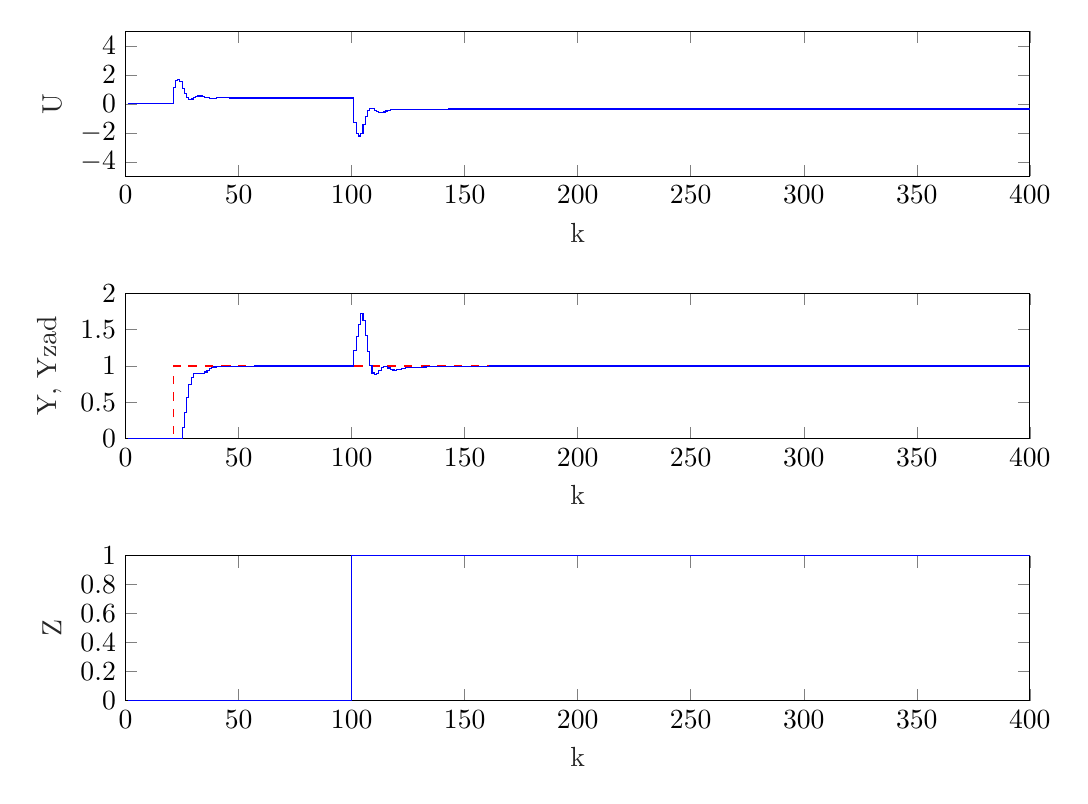
\begin{tikzpicture}

\begin{axis}[%
width=4.521in,
height=0.725in,
at={(0.758in,3.322in)},
scale only axis,
xmin=0,
xmax=400,
xlabel style={font=\color{white!15!black}},
xlabel={k},
ymin=-5,
ymax=5,
ylabel style={font=\color{white!15!black}},
ylabel={U},
axis background/.style={fill=white}
]
\addplot[const plot, color=blue, forget plot] table[row sep=crcr] {%
1	0\\
2	0\\
3	0\\
4	0\\
5	0\\
6	0\\
7	0\\
8	0\\
9	0\\
10	0\\
11	0\\
12	0\\
13	0\\
14	0\\
15	0\\
16	0\\
17	0\\
18	0\\
19	0\\
20	0\\
21	1.13124041331753\\
22	1.60739620208848\\
23	1.67029772812697\\
24	1.5088290696095\\
25	1.08258009935487\\
26	0.684037120257817\\
27	0.424015380122655\\
28	0.310055013493176\\
29	0.329911659559614\\
30	0.412055543717462\\
31	0.49284813281035\\
32	0.53826796688865\\
33	0.537912993315766\\
34	0.504308140292631\\
35	0.45877281065022\\
36	0.419410565589577\\
37	0.396275443971251\\
38	0.390196587205243\\
39	0.395737940223536\\
40	0.405530115035693\\
41	0.413556147410279\\
42	0.416831988264799\\
43	0.415363749413303\\
44	0.41100616794113\\
45	0.406084453780792\\
46	0.402349250225408\\
47	0.40052789855623\\
48	0.400422166673599\\
49	0.401311205757422\\
50	0.402400609633999\\
51	0.403135629315426\\
52	0.403312371317209\\
53	0.403020350347085\\
54	0.402499132197402\\
55	0.401993011482922\\
56	0.401657765772953\\
57	0.40153450897489\\
58	0.401575545994931\\
59	0.40169360029823\\
60	0.40180770201165\\
61	0.401870068243431\\
62	0.401871046600647\\
63	0.40182832958733\\
64	0.401770153994924\\
65	0.401720848379131\\
66	0.401693163682481\\
67	0.401687705971358\\
68	0.401697066358232\\
69	0.40171140175517\\
70	0.401722879568028\\
71	0.401727766843836\\
72	0.401726257840868\\
73	0.401720930851284\\
74	0.401714902237765\\
75	0.401710465406525\\
76	0.401708535593691\\
77	0.401708807856827\\
78	0.40171030785626\\
79	0.401711988442695\\
80	0.401713135670161\\
81	0.401713504677854\\
82	0.401713234372025\\
83	0.401712653194794\\
84	0.401712087119452\\
85	0.401711739451988\\
86	0.401711660141687\\
87	0.401711782952107\\
88	0.401711991877851\\
89	0.401712181631659\\
90	0.401712292121399\\
91	0.40171231376668\\
92	0.401712272378503\\
93	0.401712206636815\\
94	0.401712149141236\\
95	0.401712116674031\\
96	0.401712109863984\\
97	0.401712118919425\\
98	0.401712131093258\\
99	0.401712136499113\\
100	0.401712130744792\\
101	-1.2965066330836\\
102	-2.06195373752893\\
103	-2.22261849637635\\
104	-2.041788843556\\
105	-1.44928017846666\\
106	-0.873919226005589\\
107	-0.48606105540711\\
108	-0.305534856057798\\
109	-0.321846923103503\\
110	-0.434065855201892\\
111	-0.54917611835704\\
112	-0.615489711647571\\
113	-0.615322158161232\\
114	-0.565174697077588\\
115	-0.495571310547111\\
116	-0.433330003762849\\
117	-0.394035910391747\\
118	-0.379820347771811\\
119	-0.383346341509407\\
120	-0.394038203243644\\
121	-0.402965508475143\\
122	-0.405469856215254\\
123	-0.401268198875585\\
124	-0.392885862513716\\
125	-0.383666690584602\\
126	-0.376212631342341\\
127	-0.371670757137998\\
128	-0.369824982898458\\
129	-0.369656574731387\\
130	-0.369996922103697\\
131	-0.369998896396801\\
132	-0.369318835740146\\
133	-0.368048638863415\\
134	-0.366514249736603\\
135	-0.365063227897577\\
136	-0.363923342469196\\
137	-0.363157881214372\\
138	-0.36269846697638\\
139	-0.362414795806124\\
140	-0.362182035707313\\
141	-0.361921913437437\\
142	-0.36161199042742\\
143	-0.361271338107681\\
144	-0.360936489849796\\
145	-0.360640033167608\\
146	-0.360398705072651\\
147	-0.360211849849388\\
148	-0.360066980747744\\
149	-0.359947776562257\\
150	-0.359840665630096\\
151	-0.359738082637506\\
152	-0.35963841025327\\
153	-0.359543832625656\\
154	-0.359457646021309\\
155	-0.359382205546912\\
156	-0.359318021741173\\
157	-0.359263910846528\\
158	-0.359217751605217\\
159	-0.359177343373064\\
160	-0.359141009074329\\
161	-0.359107811544847\\
162	-0.359077442490809\\
163	-0.359049942196655\\
164	-0.359025412598024\\
165	-0.359003829399278\\
166	-0.358984984014495\\
167	-0.358968527354513\\
168	-0.358954060533666\\
169	-0.35894122066041\\
170	-0.358929730852197\\
171	-0.358919408212067\\
172	-0.358910141361152\\
173	-0.358901856153608\\
174	-0.35889448579854\\
175	-0.358887954122458\\
176	-0.358882172745955\\
177	-0.358877047616433\\
178	-0.358872488630207\\
179	-0.358868417291093\\
180	-0.358864769971388\\
181	-0.358861496888207\\
182	-0.358858558474696\\
183	-0.358855921196655\\
184	-0.358853554343279\\
185	-0.358851428425806\\
186	-0.358849515015792\\
187	-0.358847787406338\\
188	-0.358846221420144\\
189	-0.358844795897081\\
190	-0.358843492696187\\
191	-0.358842296297447\\
192	-0.358841193214664\\
193	-0.358840171431643\\
194	-0.358839219995547\\
195	-0.358838328801537\\
196	-0.358837488526396\\
197	-0.358836690635193\\
198	-0.35883592739107\\
199	-0.358835191827129\\
200	-0.358834477672266\\
201	-0.358833779246146\\
202	-0.358833091347337\\
203	-0.358832409155003\\
204	-0.358831728154498\\
205	-0.3588310440867\\
206	-0.358830352914149\\
207	-0.358829650795052\\
208	-0.358828934058032\\
209	-0.358828199174132\\
210	-0.358827442725943\\
211	-0.35882666137584\\
212	-0.358825851835726\\
213	-0.358825010839991\\
214	-0.358824135122237\\
215	-0.358823221395253\\
216	-0.358822266333227\\
217	-0.35882128630202\\
218	-0.358820378979023\\
219	-0.358819814589547\\
220	-0.358819776890272\\
221	-0.358820286090915\\
222	-0.358821204057572\\
223	-0.358825083440865\\
224	-0.358831051780879\\
225	-0.358837251343122\\
226	-0.358842125730213\\
227	-0.358844028092926\\
228	-0.358842780561746\\
229	-0.358839420478601\\
230	-0.358835421638723\\
231	-0.358832232291134\\
232	-0.358830656182317\\
233	-0.358830692813812\\
234	-0.35883177419307\\
235	-0.358833106068771\\
236	-0.358834031527477\\
237	-0.358834243924633\\
238	-0.358833798113299\\
239	-0.358832987516844\\
240	-0.358832164643489\\
241	-0.358831590708675\\
242	-0.358831365375492\\
243	-0.358831437630541\\
244	-0.358831669838178\\
245	-0.358831914844105\\
246	-0.358832072780391\\
247	-0.358832112697097\\
248	-0.358832061871432\\
249	-0.358831976902581\\
250	-0.358831913186682\\
251	-0.358831904660474\\
252	-0.358831958067181\\
253	-0.35883205920787\\
254	-0.35883218496858\\
255	-0.358832314771742\\
256	-0.358832437382026\\
257	-0.358832552056177\\
258	-0.358832665465396\\
259	-0.358832786922503\\
260	-0.358832924241179\\
261	-0.358833081550048\\
262	-0.358833259219618\\
263	-0.35883345522365\\
264	-0.358833666951213\\
265	-0.358833892647954\\
266	-0.358834132078323\\
267	-0.3588343864265\\
268	-0.358834657729916\\
269	-0.358834948213234\\
270	-0.358835259803231\\
271	-0.358835593943214\\
272	-0.358835951674714\\
273	-0.358836333866464\\
274	-0.358836741457212\\
275	-0.358837175619475\\
276	-0.358837637812362\\
277	-0.35883812974361\\
278	-0.358838653287701\\
279	-0.358839210407208\\
280	-0.358839803107211\\
281	-0.358840433430329\\
282	-0.358841103482413\\
283	-0.358841815471215\\
284	-0.358842571741802\\
285	-0.358843374799415\\
286	-0.358844227318485\\
287	-0.358845132142212\\
288	-0.358846092279216\\
289	-0.358847110902781\\
290	-0.358848191355488\\
291	-0.358849337159281\\
292	-0.358850552029149\\
293	-0.358851839888145\\
294	-0.358853204881924\\
295	-0.358854651392043\\
296	-0.35885618389586\\
297	-0.358857776922986\\
298	-0.358859281133196\\
299	-0.358860285016794\\
300	-0.358860496066319\\
301	-0.358859861394664\\
302	-0.358858546064972\\
303	-0.358852719767892\\
304	-0.358843575459608\\
305	-0.358833834078022\\
306	-0.358825855884666\\
307	-0.358822198514242\\
308	-0.358823276296427\\
309	-0.358827670371471\\
310	-0.358833244755784\\
311	-0.358837828488495\\
312	-0.358840154137223\\
313	-0.358840133165282\\
314	-0.358838539312572\\
315	-0.358836520144741\\
316	-0.358835057322021\\
317	-0.358834636303846\\
318	-0.358835210612128\\
319	-0.358836369145861\\
320	-0.358837595798443\\
321	-0.358838494444848\\
322	-0.358838900412504\\
323	-0.35883887258742\\
324	-0.358838604248971\\
325	-0.358838310677736\\
326	-0.358838143429977\\
327	-0.358838154941733\\
328	-0.358838311026004\\
329	-0.358838531591942\\
330	-0.358838735384866\\
331	-0.358838870792072\\
332	-0.358838925704379\\
333	-0.358838919498379\\
334	-0.358838885915156\\
335	-0.358838856162297\\
336	-0.358838848447144\\
337	-0.358838865726568\\
338	-0.358838899811669\\
339	-0.358838938213407\\
340	-0.358838970288726\\
341	-0.35883899064507\\
342	-0.358838999457132\\
343	-0.35883900061063\\
344	-0.358838999088252\\
345	-0.358838998820083\\
346	-0.358839001638426\\
347	-0.3588390073525\\
348	-0.358839014538447\\
349	-0.358839021511731\\
350	-0.358839027061692\\
351	-0.358839030758319\\
352	-0.358839032863901\\
353	-0.358839034017107\\
354	-0.358839034884058\\
355	-0.358839035916681\\
356	-0.358839037271072\\
357	-0.358839038861379\\
358	-0.358839040483056\\
359	-0.35883904193638\\
360	-0.358839043104745\\
361	-0.358839043974568\\
362	-0.358839044609693\\
363	-0.358839045105521\\
364	-0.358839045546845\\
365	-0.358839045983722\\
366	-0.358839046428073\\
367	-0.358839046865145\\
368	-0.358839047270502\\
369	-0.3588390476244\\
370	-0.3588390479192\\
371	-0.358839048159538\\
372	-0.358839048357735\\
373	-0.358839048527813\\
374	-0.358839048680835\\
375	-0.358839048822831\\
376	-0.358839048955185\\
377	-0.35883904907651\\
378	-0.358839049184784\\
379	-0.358839049278912\\
380	-0.358839049359323\\
381	-0.35883904942774\\
382	-0.358839049486507\\
383	-0.358839049537873\\
384	-0.358839049583523\\
385	-0.358839049624445\\
386	-0.358839049661073\\
387	-0.358839049693548\\
388	-0.358839049721975\\
389	-0.358839049746583\\
390	-0.358839049767759\\
391	-0.358839049786001\\
392	-0.358839049801827\\
393	-0.358839049815699\\
394	-0.358839049827987\\
395	-0.358839049838959\\
396	-0.358839049848819\\
397	-0.358839049857734\\
398	-0.358839049865868\\
399	-0.358839049873399\\
400	-0.358839049880517\\
};
\end{axis}

\begin{axis}[%
width=4.521in,
height=0.725in,
at={(0.758in,2.011in)},
scale only axis,
xmin=0,
xmax=400,
xlabel style={font=\color{white!15!black}},
xlabel={k},
ymin=0,
ymax=2,
ylabel style={font=\color{white!15!black}},
ylabel={Y, Yzad},
axis background/.style={fill=white}
]
\addplot[const plot, color=red, dashed, forget plot] table[row sep=crcr] {%
1	0\\
2	0\\
3	0\\
4	0\\
5	0\\
6	0\\
7	0\\
8	0\\
9	0\\
10	0\\
11	0\\
12	0\\
13	0\\
14	0\\
15	0\\
16	0\\
17	0\\
18	0\\
19	0\\
20	0\\
21	1\\
22	1\\
23	1\\
24	1\\
25	1\\
26	1\\
27	1\\
28	1\\
29	1\\
30	1\\
31	1\\
32	1\\
33	1\\
34	1\\
35	1\\
36	1\\
37	1\\
38	1\\
39	1\\
40	1\\
41	1\\
42	1\\
43	1\\
44	1\\
45	1\\
46	1\\
47	1\\
48	1\\
49	1\\
50	1\\
51	1\\
52	1\\
53	1\\
54	1\\
55	1\\
56	1\\
57	1\\
58	1\\
59	1\\
60	1\\
61	1\\
62	1\\
63	1\\
64	1\\
65	1\\
66	1\\
67	1\\
68	1\\
69	1\\
70	1\\
71	1\\
72	1\\
73	1\\
74	1\\
75	1\\
76	1\\
77	1\\
78	1\\
79	1\\
80	1\\
81	1\\
82	1\\
83	1\\
84	1\\
85	1\\
86	1\\
87	1\\
88	1\\
89	1\\
90	1\\
91	1\\
92	1\\
93	1\\
94	1\\
95	1\\
96	1\\
97	1\\
98	1\\
99	1\\
100	1\\
101	1\\
102	1\\
103	1\\
104	1\\
105	1\\
106	1\\
107	1\\
108	1\\
109	1\\
110	1\\
111	1\\
112	1\\
113	1\\
114	1\\
115	1\\
116	1\\
117	1\\
118	1\\
119	1\\
120	1\\
121	1\\
122	1\\
123	1\\
124	1\\
125	1\\
126	1\\
127	1\\
128	1\\
129	1\\
130	1\\
131	1\\
132	1\\
133	1\\
134	1\\
135	1\\
136	1\\
137	1\\
138	1\\
139	1\\
140	1\\
141	1\\
142	1\\
143	1\\
144	1\\
145	1\\
146	1\\
147	1\\
148	1\\
149	1\\
150	1\\
151	1\\
152	1\\
153	1\\
154	1\\
155	1\\
156	1\\
157	1\\
158	1\\
159	1\\
160	1\\
161	1\\
162	1\\
163	1\\
164	1\\
165	1\\
166	1\\
167	1\\
168	1\\
169	1\\
170	1\\
171	1\\
172	1\\
173	1\\
174	1\\
175	1\\
176	1\\
177	1\\
178	1\\
179	1\\
180	1\\
181	1\\
182	1\\
183	1\\
184	1\\
185	1\\
186	1\\
187	1\\
188	1\\
189	1\\
190	1\\
191	1\\
192	1\\
193	1\\
194	1\\
195	1\\
196	1\\
197	1\\
198	1\\
199	1\\
200	1\\
201	1\\
202	1\\
203	1\\
204	1\\
205	1\\
206	1\\
207	1\\
208	1\\
209	1\\
210	1\\
211	1\\
212	1\\
213	1\\
214	1\\
215	1\\
216	1\\
217	1\\
218	1\\
219	1\\
220	1\\
221	1\\
222	1\\
223	1\\
224	1\\
225	1\\
226	1\\
227	1\\
228	1\\
229	1\\
230	1\\
231	1\\
232	1\\
233	1\\
234	1\\
235	1\\
236	1\\
237	1\\
238	1\\
239	1\\
240	1\\
241	1\\
242	1\\
243	1\\
244	1\\
245	1\\
246	1\\
247	1\\
248	1\\
249	1\\
250	1\\
251	1\\
252	1\\
253	1\\
254	1\\
255	1\\
256	1\\
257	1\\
258	1\\
259	1\\
260	1\\
261	1\\
262	1\\
263	1\\
264	1\\
265	1\\
266	1\\
267	1\\
268	1\\
269	1\\
270	1\\
271	1\\
272	1\\
273	1\\
274	1\\
275	1\\
276	1\\
277	1\\
278	1\\
279	1\\
280	1\\
281	1\\
282	1\\
283	1\\
284	1\\
285	1\\
286	1\\
287	1\\
288	1\\
289	1\\
290	1\\
291	1\\
292	1\\
293	1\\
294	1\\
295	1\\
296	1\\
297	1\\
298	1\\
299	1\\
300	1\\
301	1\\
302	1\\
303	1\\
304	1\\
305	1\\
306	1\\
307	1\\
308	1\\
309	1\\
310	1\\
311	1\\
312	1\\
313	1\\
314	1\\
315	1\\
316	1\\
317	1\\
318	1\\
319	1\\
320	1\\
321	1\\
322	1\\
323	1\\
324	1\\
325	1\\
326	1\\
327	1\\
328	1\\
329	1\\
330	1\\
331	1\\
332	1\\
333	1\\
334	1\\
335	1\\
336	1\\
337	1\\
338	1\\
339	1\\
340	1\\
341	1\\
342	1\\
343	1\\
344	1\\
345	1\\
346	1\\
347	1\\
348	1\\
349	1\\
350	1\\
351	1\\
352	1\\
353	1\\
354	1\\
355	1\\
356	1\\
357	1\\
358	1\\
359	1\\
360	1\\
361	1\\
362	1\\
363	1\\
364	1\\
365	1\\
366	1\\
367	1\\
368	1\\
369	1\\
370	1\\
371	1\\
372	1\\
373	1\\
374	1\\
375	1\\
376	1\\
377	1\\
378	1\\
379	1\\
380	1\\
381	1\\
382	1\\
383	1\\
384	1\\
385	1\\
386	1\\
387	1\\
388	1\\
389	1\\
390	1\\
391	1\\
392	1\\
393	1\\
394	1\\
395	1\\
396	1\\
397	1\\
398	1\\
399	1\\
400	1\\
};
\addplot[const plot, color=blue, forget plot] table[row sep=crcr] {%
1	0\\
2	0\\
3	0\\
4	0\\
5	0\\
6	0\\
7	0\\
8	0\\
9	0\\
10	0\\
11	0\\
12	0\\
13	0\\
14	0\\
15	0\\
16	0\\
17	0\\
18	0\\
19	0\\
20	0\\
21	0\\
22	0\\
23	0\\
24	0\\
25	0.152830579839198\\
26	0.361723685979986\\
27	0.567813252929803\\
28	0.740934525440941\\
29	0.847095360437015\\
30	0.893658115143514\\
31	0.90255973864811\\
32	0.895570671873684\\
33	0.89163036498361\\
34	0.898990405246294\\
35	0.91685828271975\\
36	0.939887677878803\\
37	0.961615803129477\\
38	0.977621370527924\\
39	0.986602460199098\\
40	0.989773437013205\\
41	0.989641380644215\\
42	0.988689847199495\\
43	0.988533654813312\\
44	0.989704626042417\\
45	0.991892848316057\\
46	0.994401945347177\\
47	0.996573965969035\\
48	0.998037076898529\\
49	0.998753666950623\\
50	0.998924656597726\\
51	0.998838350857697\\
52	0.998740665168325\\
53	0.998766808279368\\
54	0.998937329483177\\
55	0.999196697549384\\
56	0.999464818354491\\
57	0.999678006297738\\
58	0.999808372281484\\
59	0.999862529279366\\
60	0.999867769339971\\
61	0.999855454910885\\
62	0.999848800913543\\
63	0.999857968169211\\
64	0.999881621834702\\
65	0.999912037309881\\
66	0.999940598025195\\
67	0.999961538784302\\
68	0.999973216807206\\
69	0.999977361349574\\
70	0.999977327623101\\
71	0.999976368399375\\
72	0.999976556980123\\
73	0.999978522354457\\
74	0.999981799158156\\
75	0.999985440953475\\
76	0.999988577040411\\
77	0.999990730653257\\
78	0.99999187053213\\
79	0.999992275801492\\
80	0.999992333120867\\
81	0.99999236613075\\
82	0.999992548519416\\
83	0.999992902381439\\
84	0.999993351510946\\
85	0.999993790164412\\
86	0.999994136571704\\
87	0.999994357305398\\
88	0.999994464385011\\
89	0.999994496292151\\
90	0.999994495860299\\
91	0.999994494377281\\
92	0.999994505516522\\
93	0.999994527765157\\
94	0.999994551375948\\
95	0.999994565659013\\
96	0.999994563834085\\
97	0.999994544575335\\
98	0.999994510910527\\
99	0.999994467862375\\
100	0.999994420170427\\
101	1.2132443709093\\
102	1.40256084618896\\
103	1.57062529004848\\
104	1.71981897655279\\
105	1.62282724588391\\
106	1.41995459808995\\
107	1.19950162611547\\
108	1.00932764956893\\
109	0.90409904220431\\
110	0.877513324030484\\
111	0.900523871003551\\
112	0.942914111803771\\
113	0.977464996508792\\
114	0.992017745065742\\
115	0.987595774791811\\
116	0.972113313699141\\
117	0.955412940065127\\
118	0.944546306560698\\
119	0.94203369851563\\
120	0.946612589660162\\
121	0.954962375140789\\
122	0.963635658733371\\
123	0.97034641617373\\
124	0.974346632432493\\
125	0.976122504954977\\
126	0.976751984397285\\
127	0.977282916239528\\
128	0.97835636227896\\
129	0.980119001734052\\
130	0.98235098037585\\
131	0.984683079962814\\
132	0.986789669339526\\
133	0.988495418148549\\
134	0.989787977241426\\
135	0.990766226594543\\
136	0.991566677224175\\
137	0.992302976642364\\
138	0.993035867008876\\
139	0.99377342960413\\
140	0.994490387096157\\
141	0.995152370314665\\
142	0.995734412650862\\
143	0.996228998627073\\
144	0.996644549967325\\
145	0.996998423375391\\
146	0.997309016717337\\
147	0.997590222341678\\
148	0.997849416072811\\
149	0.998088435544036\\
150	0.998306103656121\\
151	0.998500814760464\\
152	0.998672221408805\\
153	0.998821742226959\\
154	0.998952146298926\\
155	0.999066714234909\\
156	0.999168447358503\\
157	0.999259605112004\\
158	0.999341626794327\\
159	0.999415331370156\\
160	0.999481225363911\\
161	0.999539770990731\\
162	0.999591535042412\\
163	0.999637211564794\\
164	0.999677559871319\\
165	0.999713314924706\\
166	0.999745116009279\\
167	0.999773475747175\\
168	0.999798788329237\\
169	0.999821361596766\\
170	0.999841454266772\\
171	0.999859304370734\\
172	0.999875143138726\\
173	0.999889195865169\\
174	0.999901675369367\\
175	0.999912774198161\\
176	0.999922659811791\\
177	0.999931474241511\\
178	0.999939337428997\\
179	0.999946352315005\\
180	0.999952609739997\\
181	0.999958191935784\\
182	0.99996317429627\\
183	0.999967625811598\\
184	0.999971608855222\\
185	0.99997517895827\\
186	0.999978384942093\\
187	0.999981269480738\\
188	0.999983869952858\\
189	0.999986219362934\\
190	0.999988347144859\\
191	0.999990279753127\\
192	0.999992041042183\\
193	0.999993652496609\\
194	0.999995133392858\\
195	0.999996500956552\\
196	0.999997770546657\\
197	0.999998955866853\\
198	1.00000006918578\\
199	1.00000112154373\\
200	1.00000212292974\\
201	1.0000030824241\\
202	1.00000400831016\\
203	1.00000490816485\\
204	1.00000578893731\\
205	1.00000665702245\\
206	1.00000751833215\\
207	1.00000837836415\\
208	1.00000924226656\\
209	1.0000101148965\\
210	1.00001100087173\\
211	1.00001190461568\\
212	1.00001283039681\\
213	1.00001378236393\\
214	1.00001476457847\\
215	1.00001578104481\\
216	1.00001683573893\\
217	1.00001793263554\\
218	1.00001907573374\\
219	1.00002026908101\\
220	1.00002151679595\\
221	1.00002282042179\\
222	1.00002416809636\\
223	1.00002551197998\\
224	1.00002678189604\\
225	1.00002790864644\\
226	1.00002884536207\\
227	1.00002920278004\\
228	1.00002873050344\\
229	1.00002744261566\\
230	1.00002556267479\\
231	1.00002352460728\\
232	1.00002176286929\\
233	1.00002054823738\\
234	1.00001993769169\\
235	1.00001978942981\\
236	1.0000198606941\\
237	1.00001992189287\\
238	1.00001983256527\\
239	1.00001956713534\\
240	1.00001919014862\\
241	1.00001880407812\\
242	1.00001849843435\\
243	1.00001831823449\\
244	1.00001825842584\\
245	1.00001827892791\\
246	1.00001832835405\\
247	1.0000183649812\\
248	1.00001836793184\\
249	1.00001833733402\\
250	1.00001828679767\\
251	1.00001823337506\\
252	1.00001818950809\\
253	1.00001815931627\\
254	1.00001813920941\\
255	1.00001812120407\\
256	1.00001809683534\\
257	1.00001806001259\\
258	1.00001800809587\\
259	1.00001794136689\\
260	1.00001786160905\\
261	1.00001777060882\\
262	1.00001766915398\\
263	1.00001755673076\\
264	1.00001743179687\\
265	1.00001729233508\\
266	1.00001713638668\\
267	1.00001696237226\\
268	1.00001676915026\\
269	1.00001655587763\\
270	1.00001632178852\\
271	1.00001606599839\\
272	1.00001578739515\\
273	1.00001548462622\\
274	1.0000151561518\\
275	1.00001480032038\\
276	1.00001441542905\\
277	1.0000139997497\\
278	1.00001355152095\\
279	1.00001306891834\\
280	1.00001255001914\\
281	1.00001199277401\\
282	1.00001139499141\\
283	1.00001075433338\\
284	1.00001006831774\\
285	1.00000933432085\\
286	1.00000854957674\\
287	1.00000771117109\\
288	1.00000681603067\\
289	1.00000586091039\\
290	1.0000048423797\\
291	1.00000375680988\\
292	1.00000260036244\\
293	1.00000136897825\\
294	1.00000005836659\\
295	0.999998663993534\\
296	0.99999718106901\\
297	0.999995604532601\\
298	0.999993929038123\\
299	0.999992148937246\\
300	0.999990258282933\\
301	0.999988254891579\\
302	0.999986156874312\\
303	0.999984036958374\\
304	0.999982003455447\\
305	0.999980165962755\\
306	0.999978605846353\\
307	0.999977917540985\\
308	0.999978502155564\\
309	0.999980371487599\\
310	0.999983217800888\\
311	0.999986404445451\\
312	0.999989273216766\\
313	0.999991393200147\\
314	0.999992645374249\\
315	0.999993210474422\\
316	0.999993430713079\\
317	0.999993641770846\\
318	0.99999405664738\\
319	0.999994721785157\\
320	0.999995548487494\\
321	0.999996387264115\\
322	0.999997102986479\\
323	0.999997623374989\\
324	0.999997949788687\\
325	0.999998137034\\
326	0.99999825920419\\
327	0.999998378431855\\
328	0.999998527377506\\
329	0.999998707849904\\
330	0.999998901083312\\
331	0.999999082241561\\
332	0.999999232449694\\
333	0.999999344673752\\
334	0.999999423237972\\
335	0.999999479205951\\
336	0.999999524679075\\
337	0.999999568486407\\
338	0.999999614420782\\
339	0.999999661853326\\
340	0.999999707728911\\
341	0.999999748757792\\
342	0.999999782934189\\
343	0.999999810047896\\
344	0.999999831337834\\
345	0.999999848704344\\
346	0.999999863921268\\
347	0.999999878141399\\
348	0.999999891781859\\
349	0.999999904706081\\
350	0.999999916537182\\
351	0.999999926944302\\
352	0.99999993580672\\
353	0.999999943237734\\
354	0.99999994950799\\
355	0.999999954931516\\
356	0.999999959769845\\
357	0.999999964184012\\
358	0.99999996823628\\
359	0.999999971924426\\
360	0.999999975225199\\
361	0.999999978128154\\
362	0.999999980650999\\
363	0.999999982837428\\
364	0.999999984744487\\
365	0.999999986427941\\
366	0.999999987931884\\
367	0.999999989285105\\
368	0.999999990503358\\
369	0.999999991594757\\
370	0.999999992565345\\
371	0.999999993422815\\
372	0.999999994177725\\
373	0.999999994842717\\
374	0.999999995430764\\
375	0.999999995953502\\
376	0.999999996420261\\
377	0.99999999683796\\
378	0.999999997211642\\
379	0.999999997545252\\
380	0.999999997842328\\
381	0.999999998106399\\
382	0.999999998341067\\
383	0.999999998549884\\
384	0.999999998736146\\
385	0.999999998902734\\
386	0.99999999905205\\
387	0.999999999186063\\
388	0.999999999306402\\
389	0.99999999941447\\
390	0.999999999511535\\
391	0.999999999598775\\
392	0.999999999677288\\
393	0.999999999748077\\
394	0.999999999812041\\
395	0.999999999869957\\
396	0.999999999922494\\
397	0.999999999970215\\
398	1.00000000001361\\
399	1.00000000005309\\
400	1.00000000008903\\
};
\end{axis}

\begin{axis}[%
width=4.521in,
height=0.725in,
at={(0.758in,0.7in)},
scale only axis,
xmin=0,
xmax=400,
xlabel style={font=\color{white!15!black}},
xlabel={k},
ymin=0,
ymax=1,
ylabel style={font=\color{white!15!black}},
ylabel={Z},
axis background/.style={fill=white}
]
\addplot[const plot, color=blue, forget plot] table[row sep=crcr] {%
1	0\\
2	0\\
3	0\\
4	0\\
5	0\\
6	0\\
7	0\\
8	0\\
9	0\\
10	0\\
11	0\\
12	0\\
13	0\\
14	0\\
15	0\\
16	0\\
17	0\\
18	0\\
19	0\\
20	0\\
21	0\\
22	0\\
23	0\\
24	0\\
25	0\\
26	0\\
27	0\\
28	0\\
29	0\\
30	0\\
31	0\\
32	0\\
33	0\\
34	0\\
35	0\\
36	0\\
37	0\\
38	0\\
39	0\\
40	0\\
41	0\\
42	0\\
43	0\\
44	0\\
45	0\\
46	0\\
47	0\\
48	0\\
49	0\\
50	0\\
51	0\\
52	0\\
53	0\\
54	0\\
55	0\\
56	0\\
57	0\\
58	0\\
59	0\\
60	0\\
61	0\\
62	0\\
63	0\\
64	0\\
65	0\\
66	0\\
67	0\\
68	0\\
69	0\\
70	0\\
71	0\\
72	0\\
73	0\\
74	0\\
75	0\\
76	0\\
77	0\\
78	0\\
79	0\\
80	0\\
81	0\\
82	0\\
83	0\\
84	0\\
85	0\\
86	0\\
87	0\\
88	0\\
89	0\\
90	0\\
91	0\\
92	0\\
93	0\\
94	0\\
95	0\\
96	0\\
97	0\\
98	0\\
99	0\\
100	1\\
101	1\\
102	1\\
103	1\\
104	1\\
105	1\\
106	1\\
107	1\\
108	1\\
109	1\\
110	1\\
111	1\\
112	1\\
113	1\\
114	1\\
115	1\\
116	1\\
117	1\\
118	1\\
119	1\\
120	1\\
121	1\\
122	1\\
123	1\\
124	1\\
125	1\\
126	1\\
127	1\\
128	1\\
129	1\\
130	1\\
131	1\\
132	1\\
133	1\\
134	1\\
135	1\\
136	1\\
137	1\\
138	1\\
139	1\\
140	1\\
141	1\\
142	1\\
143	1\\
144	1\\
145	1\\
146	1\\
147	1\\
148	1\\
149	1\\
150	1\\
151	1\\
152	1\\
153	1\\
154	1\\
155	1\\
156	1\\
157	1\\
158	1\\
159	1\\
160	1\\
161	1\\
162	1\\
163	1\\
164	1\\
165	1\\
166	1\\
167	1\\
168	1\\
169	1\\
170	1\\
171	1\\
172	1\\
173	1\\
174	1\\
175	1\\
176	1\\
177	1\\
178	1\\
179	1\\
180	1\\
181	1\\
182	1\\
183	1\\
184	1\\
185	1\\
186	1\\
187	1\\
188	1\\
189	1\\
190	1\\
191	1\\
192	1\\
193	1\\
194	1\\
195	1\\
196	1\\
197	1\\
198	1\\
199	1\\
200	1\\
201	1\\
202	1\\
203	1\\
204	1\\
205	1\\
206	1\\
207	1\\
208	1\\
209	1\\
210	1\\
211	1\\
212	1\\
213	1\\
214	1\\
215	1\\
216	1\\
217	1\\
218	1\\
219	1\\
220	1\\
221	1\\
222	1\\
223	1\\
224	1\\
225	1\\
226	1\\
227	1\\
228	1\\
229	1\\
230	1\\
231	1\\
232	1\\
233	1\\
234	1\\
235	1\\
236	1\\
237	1\\
238	1\\
239	1\\
240	1\\
241	1\\
242	1\\
243	1\\
244	1\\
245	1\\
246	1\\
247	1\\
248	1\\
249	1\\
250	1\\
251	1\\
252	1\\
253	1\\
254	1\\
255	1\\
256	1\\
257	1\\
258	1\\
259	1\\
260	1\\
261	1\\
262	1\\
263	1\\
264	1\\
265	1\\
266	1\\
267	1\\
268	1\\
269	1\\
270	1\\
271	1\\
272	1\\
273	1\\
274	1\\
275	1\\
276	1\\
277	1\\
278	1\\
279	1\\
280	1\\
281	1\\
282	1\\
283	1\\
284	1\\
285	1\\
286	1\\
287	1\\
288	1\\
289	1\\
290	1\\
291	1\\
292	1\\
293	1\\
294	1\\
295	1\\
296	1\\
297	1\\
298	1\\
299	1\\
300	1\\
301	1\\
302	1\\
303	1\\
304	1\\
305	1\\
306	1\\
307	1\\
308	1\\
309	1\\
310	1\\
311	1\\
312	1\\
313	1\\
314	1\\
315	1\\
316	1\\
317	1\\
318	1\\
319	1\\
320	1\\
321	1\\
322	1\\
323	1\\
324	1\\
325	1\\
326	1\\
327	1\\
328	1\\
329	1\\
330	1\\
331	1\\
332	1\\
333	1\\
334	1\\
335	1\\
336	1\\
337	1\\
338	1\\
339	1\\
340	1\\
341	1\\
342	1\\
343	1\\
344	1\\
345	1\\
346	1\\
347	1\\
348	1\\
349	1\\
350	1\\
351	1\\
352	1\\
353	1\\
354	1\\
355	1\\
356	1\\
357	1\\
358	1\\
359	1\\
360	1\\
361	1\\
362	1\\
363	1\\
364	1\\
365	1\\
366	1\\
367	1\\
368	1\\
369	1\\
370	1\\
371	1\\
372	1\\
373	1\\
374	1\\
375	1\\
376	1\\
377	1\\
378	1\\
379	1\\
380	1\\
381	1\\
382	1\\
383	1\\
384	1\\
385	1\\
386	1\\
387	1\\
388	1\\
389	1\\
390	1\\
391	1\\
392	1\\
393	1\\
394	1\\
395	1\\
396	1\\
397	1\\
398	1\\
399	1\\
400	1\\
};
\end{axis}
\end{tikzpicture}%
	\label{5zprzebieg}
\end{figure}

\section{Dla zakłócenia zmiennego sinusoidalnie}

Zasymulowano przebiegi procesu dla zmiany wartości zakłócenia mierzalnego w chwili odpowiadającej 100-nej próbce symulacji na sygnał sinusoidalny o amplitudzie \num{0.2}. Symulacje uruchomiono w w dwóch trybach pracy algorytmu DMC.



\subsection{Bez uwzględniania zakłóceń}

W trybie pracy algorytmu bez uwzględniania zakłóceń otrzymano wskaźnik jakości $e$~=~\num{12.3087}. Przebieg przedstawiono na rysunku \ref{6przebieg}

\begin{figure}
	
	\centering
	\caption{ Przebieg symulacji algorytmu DMC dla zakłócenia zmiennego sinusoidalnie bez uwzględniania zakłóceń }
	% This file was created by matlab2tikz.
%
%The latest updates can be retrieved from
%  http://www.mathworks.com/matlabcentral/fileexchange/22022-matlab2tikz-matlab2tikz
%where you can also make suggestions and rate matlab2tikz.
%
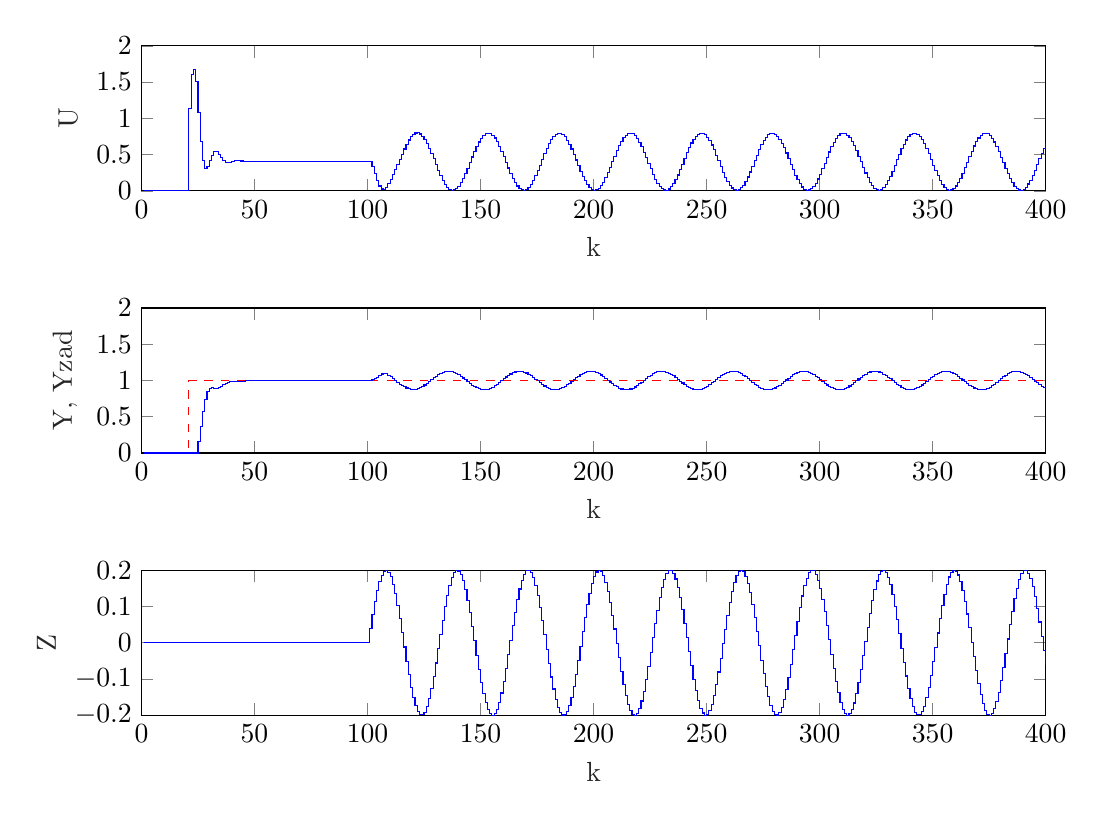
\begin{tikzpicture}

\begin{axis}[%
width=4.521in,
height=0.725in,
at={(0.758in,3.322in)},
scale only axis,
xmin=0,
xmax=400,
xlabel style={font=\color{white!15!black}},
xlabel={k},
ymin=0,
ymax=2,
ylabel style={font=\color{white!15!black}},
ylabel={U},
axis background/.style={fill=white}
]
\addplot[const plot, color=blue, forget plot] table[row sep=crcr] {%
1	0\\
2	0\\
3	0\\
4	0\\
5	0\\
6	0\\
7	0\\
8	0\\
9	0\\
10	0\\
11	0\\
12	0\\
13	0\\
14	0\\
15	0\\
16	0\\
17	0\\
18	0\\
19	0\\
20	0\\
21	1.13124041331753\\
22	1.60739620208848\\
23	1.67029772812697\\
24	1.5088290696095\\
25	1.08258009935487\\
26	0.684037120257817\\
27	0.424015380122655\\
28	0.310055013493176\\
29	0.329911659559614\\
30	0.412055543717462\\
31	0.49284813281035\\
32	0.53826796688865\\
33	0.537912993315766\\
34	0.504308140292631\\
35	0.45877281065022\\
36	0.419410565589577\\
37	0.396275443971251\\
38	0.390196587205243\\
39	0.395737940223536\\
40	0.405530115035693\\
41	0.413556147410279\\
42	0.416831988264799\\
43	0.415363749413303\\
44	0.41100616794113\\
45	0.406084453780792\\
46	0.402349250225408\\
47	0.40052789855623\\
48	0.400422166673599\\
49	0.401311205757422\\
50	0.402400609633999\\
51	0.403135629315426\\
52	0.403312371317209\\
53	0.403020350347085\\
54	0.402499132197402\\
55	0.401993011482922\\
56	0.401657765772953\\
57	0.40153450897489\\
58	0.401575545994931\\
59	0.40169360029823\\
60	0.40180770201165\\
61	0.401870068243431\\
62	0.401871046600647\\
63	0.40182832958733\\
64	0.401770153994924\\
65	0.401720848379131\\
66	0.401693163682481\\
67	0.401687705971358\\
68	0.401697066358232\\
69	0.40171140175517\\
70	0.401722879568028\\
71	0.401727766843836\\
72	0.401726257840868\\
73	0.401720930851284\\
74	0.401714902237765\\
75	0.401710465406525\\
76	0.401708535593691\\
77	0.401708807856827\\
78	0.40171030785626\\
79	0.401711988442695\\
80	0.401713135670161\\
81	0.401713504677854\\
82	0.401713234372025\\
83	0.401712653194794\\
84	0.401712087119452\\
85	0.401711739451988\\
86	0.401711660141687\\
87	0.401711782952107\\
88	0.401711991877851\\
89	0.401712181631659\\
90	0.401712292121399\\
91	0.40171231376668\\
92	0.401712272378503\\
93	0.401712206636815\\
94	0.401712149141236\\
95	0.401712116674031\\
96	0.401712109863984\\
97	0.401712118919425\\
98	0.401712131093258\\
99	0.401712136499113\\
100	0.401712130744792\\
101	0.401712114581669\\
102	0.334235295364013\\
103	0.2390343889258\\
104	0.143935098022229\\
105	0.0662976248260884\\
106	0.0255747278831896\\
107	0.0227085536006074\\
108	0.0503631547944995\\
109	0.0991979273976707\\
110	0.159444836804326\\
111	0.224891277756517\\
112	0.292813223027465\\
113	0.362441718882142\\
114	0.433642449231152\\
115	0.505562759706866\\
116	0.576108472576573\\
117	0.642174627887164\\
118	0.700215593912494\\
119	0.746920992479067\\
120	0.779723885135827\\
121	0.797031795494936\\
122	0.798224823517292\\
123	0.783510614938869\\
124	0.753742233375495\\
125	0.710272563829294\\
126	0.654867854582507\\
127	0.58966678082823\\
128	0.517152990292335\\
129	0.440110251554892\\
130	0.361543366322557\\
131	0.28456433264335\\
132	0.212255505643744\\
133	0.147526709075593\\
134	0.0929819233198008\\
135	0.0508061733855565\\
136	0.0226775599909048\\
137	0.00970511872147983\\
138	0.0123911417639461\\
139	0.0306163846595809\\
140	0.0636472807968308\\
141	0.110164968976698\\
142	0.168316022288995\\
143	0.235784119868662\\
144	0.309880741948237\\
145	0.387651658828556\\
146	0.465994863480688\\
147	0.541784868581303\\
148	0.611998000911901\\
149	0.673833415763506\\
150	0.724824910136951\\
151	0.76293913322666\\
152	0.786656411048066\\
153	0.795031094710474\\
154	0.787729109409936\\
155	0.765041228752116\\
156	0.727871519925772\\
157	0.677701374692524\\
158	0.6165305182971\\
159	0.546797323987093\\
160	0.47128160592513\\
161	0.392993775971781\\
162	0.315054798670057\\
163	0.240571743255718\\
164	0.172513900767026\\
165	0.113594405337491\\
166	0.0661620751216979\\
167	0.0321077796568143\\
168	0.0127890624508853\\
169	0.00897602199317402\\
170	0.020820608935247\\
171	0.0478505648888333\\
172	0.088988246151833\\
173	0.14259358312961\\
174	0.206529463264589\\
175	0.278246930688012\\
176	0.354886805430513\\
177	0.433393670401413\\
178	0.510637681463889\\
179	0.583539344299978\\
180	0.649192283683627\\
181	0.704979110913078\\
182	0.748675770303983\\
183	0.778540204881413\\
184	0.793381806471504\\
185	0.792608881398111\\
186	0.776252239413078\\
187	0.744963965386782\\
188	0.699991422695134\\
189	0.643127524700198\\
190	0.576639256856359\\
191	0.503177299059485\\
192	0.425670351326792\\
193	0.347208375716671\\
194	0.270919409263848\\
195	0.19984485900324\\
196	0.136818250668902\\
197	0.0843522649689548\\
198	0.0445385649409795\\
199	0.0189644079550476\\
200	0.00864936678234701\\
201	0.0140046824626434\\
202	0.0348168694448468\\
203	0.0702562266124021\\
204	0.118909914885383\\
205	0.178838282698892\\
206	0.247652193837894\\
207	0.32260827481125\\
208	0.400718284552564\\
209	0.478868246223199\\
210	0.553942591708697\\
211	0.622948369559626\\
212	0.683134564598481\\
213	0.732101772296593\\
214	0.767897855549882\\
215	0.789095770319742\\
216	0.794850457476509\\
217	0.784932513000496\\
218	0.759737271286672\\
219	0.720268949246041\\
220	0.668100859560196\\
221	0.605312757395917\\
222	0.534407921097868\\
223	0.458210510739775\\
224	0.379758991886682\\
225	0.302182596493468\\
226	0.228575357740125\\
227	0.161873214520335\\
228	0.104735471037573\\
229	0.0594390395911265\\
230	0.0277884046652801\\
231	0.0110440870673605\\
232	0.00987295215752237\\
233	0.0243217517293651\\
234	0.0538150234321128\\
235	0.0971777140479765\\
236	0.152681693225108\\
237	0.218114461841866\\
238	0.290867358364439\\
239	0.368039678694765\\
240	0.446554485881807\\
241	0.523281414217985\\
242	0.595161526893795\\
243	0.659329251313597\\
244	0.713226558419802\\
245	0.754704871631463\\
246	0.782110672883595\\
247	0.794351405534735\\
248	0.790939043088506\\
249	0.772009573099859\\
250	0.738317604062009\\
251	0.691206299608933\\
252	0.632553835215928\\
253	0.564698514765994\\
254	0.490345538308765\\
255	0.412459143759277\\
256	0.334144426120043\\
257	0.258523546460307\\
258	0.188611264335441\\
259	0.127194753366711\\
260	0.0767224892180033\\
261	0.0392066384976454\\
262	0.0161428399609795\\
263	0.00845057676541253\\
264	0.0164365178775388\\
265	0.0397822908440518\\
266	0.0775571737384079\\
267	0.128255200251305\\
268	0.189855198372299\\
269	0.259901368764616\\
270	0.335601190173868\\
271	0.413936748591808\\
272	0.4917850518725\\
273	0.566042533353708\\
274	0.633748781041464\\
275	0.69220455974909\\
276	0.739079421045906\\
277	0.77250461092451\\
278	0.79114757120594\\
279	0.794265064503145\\
280	0.781732804791574\\
281	0.75405041230407\\
282	0.712321495224436\\
283	0.658209652276577\\
284	0.593872150262119\\
285	0.521873920621949\\
286	0.445085303708022\\
287	0.366567617374191\\
288	0.289451111899039\\
289	0.216810176787778\\
290	0.151540774561792\\
291	0.0962449878640206\\
292	0.0531272826245305\\
293	0.0239066229486957\\
294	0.00974794143166188\\
295	0.0112156969620783\\
296	0.0282513715186682\\
297	0.0601758030966688\\
298	0.105716262945111\\
299	0.163057200168537\\
300	0.229912632429163\\
301	0.303617276120156\\
302	0.381232793290691\\
303	0.459664925247105\\
304	0.535787009633834\\
305	0.606564431000964\\
306	0.669175540633437\\
307	0.721124161112345\\
308	0.760339093189237\\
309	0.785256773125997\\
310	0.794883679886671\\
311	0.788835972179991\\
312	0.767354792390088\\
313	0.731296617089881\\
314	0.682099065180771\\
315	0.621723550302131\\
316	0.55257707060558\\
317	0.477416255926487\\
318	0.39923748936748\\
319	0.32115747209571\\
320	0.246288984790514\\
321	0.177616795072957\\
322	0.11787865947241\\
323	0.0694561685167154\\
324	0.034279791350528\\
325	0.013751908682509\\
326	0.00869090341773893\\
327	0.0192985368458738\\
328	0.0451519089936488\\
329	0.085220321754142\\
330	0.13790637139168\\
331	0.201109632034122\\
332	0.272310391846315\\
333	0.348670104419918\\
334	0.427144551410107\\
335	0.504605205343635\\
336	0.57796395423722\\
337	0.644296215393767\\
338	0.700957529891402\\
339	0.745688989258491\\
340	0.776707291196853\\
341	0.792775834143517\\
342	0.793254016464086\\
343	0.778122774997156\\
344	0.747985344894957\\
345	0.704043210497858\\
346	0.648048205987048\\
347	0.582232675367318\\
348	0.509220476036542\\
349	0.431922373920278\\
350	0.353420000430134\\
351	0.276842997525196\\
352	0.20524424873227\\
353	0.141478170286089\\
354	0.0880869145467008\\
355	0.0471990224060222\\
356	0.0204445650879757\\
357	0.00889015836454157\\
358	0.0129964399604433\\
359	0.0325997053853986\\
360	0.0669184343153632\\
361	0.114584447338314\\
362	0.173697450945774\\
363	0.241900796235197\\
364	0.316475431063621\\
365	0.394448300076565\\
366	0.472710871044376\\
367	0.548143062234197\\
368	0.617737630223725\\
369	0.678720059206948\\
370	0.728659172183642\\
371	0.765564054313876\\
372	0.78796342440949\\
373	0.794964290271864\\
374	0.786287549472819\\
375	0.762279116287779\\
376	0.723896131185407\\
377	0.672668802657736\\
378	0.610639402636554\\
379	0.540280847556268\\
380	0.46439811097937\\
381	0.386016398152041\\
382	0.308260540617524\\
383	0.234230419043448\\
384	0.166877380761845\\
385	0.108886578864567\\
386	0.0625699236230218\\
387	0.0297739139213382\\
388	0.0118060231728269\\
389	0.00938257448095886\\
390	0.0226001830977192\\
391	0.050931904678384\\
392	0.0932482428896748\\
393	0.14786217886423\\
394	0.212596427319152\\
395	0.284870238049415\\
396	0.36180228229452\\
397	0.44032552222361\\
398	0.51730948405519\\
399	0.589685060168019\\
400	0.654566864736822\\
};
\end{axis}

\begin{axis}[%
width=4.521in,
height=0.725in,
at={(0.758in,2.011in)},
scale only axis,
xmin=0,
xmax=400,
xlabel style={font=\color{white!15!black}},
xlabel={k},
ymin=0,
ymax=2,
ylabel style={font=\color{white!15!black}},
ylabel={Y, Yzad},
axis background/.style={fill=white}
]
\addplot[const plot, color=red, dashed, forget plot] table[row sep=crcr] {%
1	0\\
2	0\\
3	0\\
4	0\\
5	0\\
6	0\\
7	0\\
8	0\\
9	0\\
10	0\\
11	0\\
12	0\\
13	0\\
14	0\\
15	0\\
16	0\\
17	0\\
18	0\\
19	0\\
20	0\\
21	1\\
22	1\\
23	1\\
24	1\\
25	1\\
26	1\\
27	1\\
28	1\\
29	1\\
30	1\\
31	1\\
32	1\\
33	1\\
34	1\\
35	1\\
36	1\\
37	1\\
38	1\\
39	1\\
40	1\\
41	1\\
42	1\\
43	1\\
44	1\\
45	1\\
46	1\\
47	1\\
48	1\\
49	1\\
50	1\\
51	1\\
52	1\\
53	1\\
54	1\\
55	1\\
56	1\\
57	1\\
58	1\\
59	1\\
60	1\\
61	1\\
62	1\\
63	1\\
64	1\\
65	1\\
66	1\\
67	1\\
68	1\\
69	1\\
70	1\\
71	1\\
72	1\\
73	1\\
74	1\\
75	1\\
76	1\\
77	1\\
78	1\\
79	1\\
80	1\\
81	1\\
82	1\\
83	1\\
84	1\\
85	1\\
86	1\\
87	1\\
88	1\\
89	1\\
90	1\\
91	1\\
92	1\\
93	1\\
94	1\\
95	1\\
96	1\\
97	1\\
98	1\\
99	1\\
100	1\\
101	1\\
102	1\\
103	1\\
104	1\\
105	1\\
106	1\\
107	1\\
108	1\\
109	1\\
110	1\\
111	1\\
112	1\\
113	1\\
114	1\\
115	1\\
116	1\\
117	1\\
118	1\\
119	1\\
120	1\\
121	1\\
122	1\\
123	1\\
124	1\\
125	1\\
126	1\\
127	1\\
128	1\\
129	1\\
130	1\\
131	1\\
132	1\\
133	1\\
134	1\\
135	1\\
136	1\\
137	1\\
138	1\\
139	1\\
140	1\\
141	1\\
142	1\\
143	1\\
144	1\\
145	1\\
146	1\\
147	1\\
148	1\\
149	1\\
150	1\\
151	1\\
152	1\\
153	1\\
154	1\\
155	1\\
156	1\\
157	1\\
158	1\\
159	1\\
160	1\\
161	1\\
162	1\\
163	1\\
164	1\\
165	1\\
166	1\\
167	1\\
168	1\\
169	1\\
170	1\\
171	1\\
172	1\\
173	1\\
174	1\\
175	1\\
176	1\\
177	1\\
178	1\\
179	1\\
180	1\\
181	1\\
182	1\\
183	1\\
184	1\\
185	1\\
186	1\\
187	1\\
188	1\\
189	1\\
190	1\\
191	1\\
192	1\\
193	1\\
194	1\\
195	1\\
196	1\\
197	1\\
198	1\\
199	1\\
200	1\\
201	1\\
202	1\\
203	1\\
204	1\\
205	1\\
206	1\\
207	1\\
208	1\\
209	1\\
210	1\\
211	1\\
212	1\\
213	1\\
214	1\\
215	1\\
216	1\\
217	1\\
218	1\\
219	1\\
220	1\\
221	1\\
222	1\\
223	1\\
224	1\\
225	1\\
226	1\\
227	1\\
228	1\\
229	1\\
230	1\\
231	1\\
232	1\\
233	1\\
234	1\\
235	1\\
236	1\\
237	1\\
238	1\\
239	1\\
240	1\\
241	1\\
242	1\\
243	1\\
244	1\\
245	1\\
246	1\\
247	1\\
248	1\\
249	1\\
250	1\\
251	1\\
252	1\\
253	1\\
254	1\\
255	1\\
256	1\\
257	1\\
258	1\\
259	1\\
260	1\\
261	1\\
262	1\\
263	1\\
264	1\\
265	1\\
266	1\\
267	1\\
268	1\\
269	1\\
270	1\\
271	1\\
272	1\\
273	1\\
274	1\\
275	1\\
276	1\\
277	1\\
278	1\\
279	1\\
280	1\\
281	1\\
282	1\\
283	1\\
284	1\\
285	1\\
286	1\\
287	1\\
288	1\\
289	1\\
290	1\\
291	1\\
292	1\\
293	1\\
294	1\\
295	1\\
296	1\\
297	1\\
298	1\\
299	1\\
300	1\\
301	1\\
302	1\\
303	1\\
304	1\\
305	1\\
306	1\\
307	1\\
308	1\\
309	1\\
310	1\\
311	1\\
312	1\\
313	1\\
314	1\\
315	1\\
316	1\\
317	1\\
318	1\\
319	1\\
320	1\\
321	1\\
322	1\\
323	1\\
324	1\\
325	1\\
326	1\\
327	1\\
328	1\\
329	1\\
330	1\\
331	1\\
332	1\\
333	1\\
334	1\\
335	1\\
336	1\\
337	1\\
338	1\\
339	1\\
340	1\\
341	1\\
342	1\\
343	1\\
344	1\\
345	1\\
346	1\\
347	1\\
348	1\\
349	1\\
350	1\\
351	1\\
352	1\\
353	1\\
354	1\\
355	1\\
356	1\\
357	1\\
358	1\\
359	1\\
360	1\\
361	1\\
362	1\\
363	1\\
364	1\\
365	1\\
366	1\\
367	1\\
368	1\\
369	1\\
370	1\\
371	1\\
372	1\\
373	1\\
374	1\\
375	1\\
376	1\\
377	1\\
378	1\\
379	1\\
380	1\\
381	1\\
382	1\\
383	1\\
384	1\\
385	1\\
386	1\\
387	1\\
388	1\\
389	1\\
390	1\\
391	1\\
392	1\\
393	1\\
394	1\\
395	1\\
396	1\\
397	1\\
398	1\\
399	1\\
400	1\\
};
\addplot[const plot, color=blue, forget plot] table[row sep=crcr] {%
1	0\\
2	0\\
3	0\\
4	0\\
5	0\\
6	0\\
7	0\\
8	0\\
9	0\\
10	0\\
11	0\\
12	0\\
13	0\\
14	0\\
15	0\\
16	0\\
17	0\\
18	0\\
19	0\\
20	0\\
21	0\\
22	0\\
23	0\\
24	0\\
25	0.152830579839198\\
26	0.361723685979986\\
27	0.567813252929803\\
28	0.740934525440941\\
29	0.847095360437015\\
30	0.893658115143514\\
31	0.90255973864811\\
32	0.895570671873684\\
33	0.89163036498361\\
34	0.898990405246294\\
35	0.91685828271975\\
36	0.939887677878803\\
37	0.961615803129477\\
38	0.977621370527924\\
39	0.986602460199098\\
40	0.989773437013205\\
41	0.989641380644215\\
42	0.988689847199495\\
43	0.988533654813312\\
44	0.989704626042417\\
45	0.991892848316057\\
46	0.994401945347177\\
47	0.996573965969035\\
48	0.998037076898529\\
49	0.998753666950623\\
50	0.998924656597726\\
51	0.998838350857697\\
52	0.998740665168325\\
53	0.998766808279368\\
54	0.998937329483177\\
55	0.999196697549384\\
56	0.999464818354491\\
57	0.999678006297738\\
58	0.999808372281484\\
59	0.999862529279366\\
60	0.999867769339971\\
61	0.999855454910885\\
62	0.999848800913543\\
63	0.999857968169211\\
64	0.999881621834702\\
65	0.999912037309881\\
66	0.999940598025195\\
67	0.999961538784302\\
68	0.999973216807206\\
69	0.999977361349574\\
70	0.999977327623101\\
71	0.999976368399375\\
72	0.999976556980123\\
73	0.999978522354457\\
74	0.999981799158156\\
75	0.999985440953475\\
76	0.999988577040411\\
77	0.999990730653257\\
78	0.99999187053213\\
79	0.999992275801492\\
80	0.999992333120867\\
81	0.99999236613075\\
82	0.999992548519416\\
83	0.999992902381439\\
84	0.999993351510946\\
85	0.999993790164412\\
86	0.999994136571704\\
87	0.999994357305398\\
88	0.999994464385011\\
89	0.999994496292151\\
90	0.999994495860299\\
91	0.999994494377281\\
92	0.999994505516522\\
93	0.999994527765157\\
94	0.999994551375948\\
95	0.999994565659013\\
96	0.999994563834085\\
97	0.999994544575335\\
98	0.999994510910527\\
99	0.999994467862375\\
100	0.999994420170427\\
101	0.999994370909295\\
102	1.00846756814737\\
103	1.02412524042148\\
104	1.04549873740651\\
105	1.07098615417743\\
106	1.0897894869801\\
107	1.09695204608207\\
108	1.09148974686446\\
109	1.07482345376639\\
110	1.05099280528335\\
111	1.0240726379727\\
112	0.997106822830562\\
113	0.971940429321492\\
114	0.949265271494161\\
115	0.929190730356925\\
116	0.911763172898169\\
117	0.897237902125641\\
118	0.886145599729037\\
119	0.879160275186301\\
120	0.876892346374106\\
121	0.879713998401527\\
122	0.887662570353424\\
123	0.900434028800379\\
124	0.917441234462095\\
125	0.937898460658789\\
126	0.960901757791112\\
127	0.98548850360104\\
128	1.0106745836872\\
129	1.03547746195109\\
130	1.05893570747977\\
131	1.08013275997311\\
132	1.09822753530338\\
133	1.11248968877153\\
134	1.12233470367997\\
135	1.12735367004439\\
136	1.12733400610924\\
137	1.1222694285396\\
138	1.11235929446379\\
139	1.09799855160112\\
140	1.07975990052392\\
141	1.05836963742826\\
142	1.0346783377447\\
143	1.00962731998219\\
144	0.984211811732718\\
145	0.959441906336624\\
146	0.936302648672162\\
147	0.915714805896407\\
148	0.898497980345131\\
149	0.885337675649939\\
150	0.876757747820665\\
151	0.87309940097526\\
152	0.87450756758343\\
153	0.880925180462769\\
154	0.892095518043524\\
155	0.907572492709888\\
156	0.926738455234154\\
157	0.948828807409089\\
158	0.972962454691947\\
159	0.998176900080328\\
160	1.02346659118666\\
161	1.04782299602912\\
162	1.07027480826367\\
163	1.0899266742636\\
164	1.10599489310515\\
165	1.11783866284971\\
166	1.12498562633376\\
167	1.12715069876355\\
168	1.12424742812056\\
169	1.11639143703251\\
170	1.10389580984113\\
171	1.08725860897402\\
172	1.06714301795446\\
173	1.04435090210635\\
174	1.01979084048842\\
175	0.994441903229234\\
176	0.969314618296533\\
177	0.945410683951149\\
178	0.923683033200544\\
179	0.90499784250252\\
180	0.890099999381749\\
181	0.879583405648838\\
182	0.873867300082941\\
183	0.87317954444952\\
184	0.877547539133908\\
185	0.886797130530064\\
186	0.900559553743016\\
187	0.918286133835661\\
188	0.939270159544737\\
189	0.962675057441526\\
190	0.987567743325218\\
191	1.01295582122954\\
192	1.03782714702727\\
193	1.06119017934828\\
194	1.08211350914147\\
195	1.09976299195905\\
196	1.11343500261617\\
197	1.12258448646869\\
198	1.12684668899436\\
199	1.12605169738803\\
200	1.12023121444303\\
201	1.10961729466431\\
202	1.09463309299939\\
203	1.07587599500484\\
204	1.05409380099472\\
205	1.03015491363343\\
206	1.00501371749964\\
207	0.979672530828834\\
208	0.955141646298545\\
209	0.93239905390413\\
210	0.912351451646891\\
211	0.89579809841531\\
212	0.883398950130936\\
213	0.875648349470253\\
214	0.872855318070408\\
215	0.8751312369065\\
216	0.882385405985153\\
217	0.894328660375589\\
218	0.910484898418745\\
219	0.930210062521374\\
220	0.952717815831076\\
221	0.977110888476762\\
222	1.00241683807791\\
223	1.02762679487319\\
224	1.05173569387671\\
225	1.07378236413806\\
226	1.09288786616339\\
227	1.10829016584793\\
228	1.11937498009483\\
229	1.12570038196096\\
230	1.1270143644332\\
231	1.12326489694906\\
232	1.11460180714353\\
233	1.10137066079897\\
234	1.08409894590141\\
235	1.06347506064144\\
236	1.04032096132319\\
237	1.01555949800297\\
238	0.990177690182373\\
239	0.965187397611719\\
240	0.941584954854863\\
241	0.920311400957579\\
242	0.902214916390749\\
243	0.888016980815316\\
244	0.878283606190112\\
245	0.87340278650983\\
246	0.873569051841418\\
247	0.878775731955199\\
248	0.888815231775185\\
249	0.90328730687906\\
250	0.921615012474442\\
251	0.943067694883721\\
252	0.966790113042385\\
253	0.991836531061098\\
254	1.01720842252499\\
255	1.04189428178203\\
256	1.06490995309411\\
257	1.08533786835933\\
258	1.10236362851188\\
259	1.11530847043164\\
260	1.12365632570349\\
261	1.12707439323494\\
262	1.12542640608237\\
263	1.11877806374181\\
264	1.10739441320076\\
265	1.09172928287598\\
266	1.07240719039432\\
267	1.05019844532511\\
268	1.02598843940275\\
269	1.00074234860858\\
270	0.975466654438754\\
271	0.951169018482647\\
272	0.92881811003964\\
273	0.909304988325098\\
274	0.893407578805095\\
275	0.88175965983456\\
276	0.874825595969611\\
277	0.872881825240674\\
278	0.876005838431606\\
279	0.884073089738624\\
280	0.896761961986487\\
281	0.913566588465848\\
282	0.933817020230242\\
283	0.956705934844739\\
284	0.981320821787769\\
285	1.00668036137025\\
286	1.03177354685556\\
287	1.05559999010362\\
288	1.07720980388108\\
289	1.09574147085762\\
290	1.11045618957281\\
291	1.12076732810955\\
292	1.12626381124908\\
293	1.12672650873526\\
294	1.12213697129903\\
295	1.11267816616442\\
296	1.09872718271368\\
297	1.08084019911341\\
298	1.05973030923506\\
299	1.0362390938407\\
300	1.01130306940141\\
301	0.985916352128886\\
302	0.961091025848729\\
303	0.937816794218676\\
304	0.917021526537232\\
305	0.899534267936835\\
306	0.886052188021748\\
307	0.877112785794239\\
308	0.873072481651674\\
309	0.874092400348387\\
310	0.880131931991292\\
311	0.890950338331847\\
312	0.906116337171324\\
313	0.925025295364656\\
314	0.946923342667026\\
315	0.970937438554292\\
316	0.996110189504144\\
317	1.02143802367071\\
318	1.04591119986754\\
319	1.06855405788774\\
320	1.08846390837952\\
321	1.10484701485248\\
322	1.11705023503116\\
323	1.12458706014706\\
324	1.12715701300522\\
325	1.12465762998774\\
326	1.11718854807855\\
327	1.10504753341758\\
328	1.08871860982925\\
329	1.06885276114891\\
330	1.04624197732578\\
331	1.02178767946545\\
332	0.996464782773813\\
333	0.971282830001139\\
334	0.947245744628957\\
335	0.925311808060194\\
336	0.906355456231456\\
337	0.891132418652912\\
338	0.880249589727547\\
339	0.874140833586369\\
340	0.873049687118955\\
341	0.87701965082978\\
342	0.885892454601059\\
343	0.899314367473909\\
344	0.916750299856761\\
345	0.937505135916384\\
346	0.960751445678871\\
347	0.985562472046567\\
348	1.01094907765433\\
349	1.03589917862562\\
350	1.05941809314088\\
351	1.08056819625322\\
352	1.098506300038\\
353	1.11251726884294\\
354	1.12204252949913\\
355	1.12670233987682\\
356	1.12631092800755\\
357	1.12088389822417\\
358	1.11063760906137\\
359	1.09598054771972\\
360	1.07749704496748\\
361	1.05592397971601\\
362	1.03212140198339\\
363	1.00703824541545\\
364	0.981674496296792\\
365	0.957041327253833\\
366	0.934120784993076\\
367	0.913826639197481\\
368	0.896967953412166\\
369	0.884216830233491\\
370	0.876081616699184\\
371	0.872886638096041\\
372	0.874759268134281\\
373	0.881624850959779\\
374	0.893209677447466\\
375	0.909051897120418\\
376	0.928519930670865\\
377	0.950837649034038\\
378	0.975115315204665\\
379	1.00038505524357\\
380	1.02563944435729\\
381	1.04987166974545\\
382	1.07211566904993\\
383	1.09148464421251\\
384	1.107206415315\\
385	1.11865420495579\\
386	1.12537162588696\\
387	1.12709087573358\\
388	1.12374341342932\\
389	1.11546269173243\\
390	1.10257883688542\\
391	1.0856054875235\\
392	1.06521931752312\\
393	1.04223305914983\\
394	1.01756310198761\\
395	0.992192959377957\\
396	0.967134058846649\\
397	0.943385419679988\\
398	0.921893825178462\\
399	0.903516077394291\\
400	0.888984839137397\\
};
\end{axis}

\begin{axis}[%
width=4.521in,
height=0.725in,
at={(0.758in,0.7in)},
scale only axis,
xmin=0,
xmax=400,
xlabel style={font=\color{white!15!black}},
xlabel={k},
ymin=-0.2,
ymax=0.2,
ylabel style={font=\color{white!15!black}},
ylabel={Z},
axis background/.style={fill=white}
]
\addplot[const plot, color=blue, forget plot] table[row sep=crcr] {%
1	0\\
2	0\\
3	0\\
4	0\\
5	0\\
6	0\\
7	0\\
8	0\\
9	0\\
10	0\\
11	0\\
12	0\\
13	0\\
14	0\\
15	0\\
16	0\\
17	0\\
18	0\\
19	0\\
20	0\\
21	0\\
22	0\\
23	0\\
24	0\\
25	0\\
26	0\\
27	0\\
28	0\\
29	0\\
30	0\\
31	0\\
32	0\\
33	0\\
34	0\\
35	0\\
36	0\\
37	0\\
38	0\\
39	0\\
40	0\\
41	0\\
42	0\\
43	0\\
44	0\\
45	0\\
46	0\\
47	0\\
48	0\\
49	0\\
50	0\\
51	0\\
52	0\\
53	0\\
54	0\\
55	0\\
56	0\\
57	0\\
58	0\\
59	0\\
60	0\\
61	0\\
62	0\\
63	0\\
64	0\\
65	0\\
66	0\\
67	0\\
68	0\\
69	0\\
70	0\\
71	0\\
72	0\\
73	0\\
74	0\\
75	0\\
76	0\\
77	0\\
78	0\\
79	0\\
80	0\\
81	0\\
82	0\\
83	0\\
84	0\\
85	0\\
86	0\\
87	0\\
88	0\\
89	0\\
90	0\\
91	0\\
92	0\\
93	0\\
94	0\\
95	0\\
96	0\\
97	0\\
98	0\\
99	0\\
100	0\\
101	0.0397338661590122\\
102	0.0778836684617301\\
103	0.112928494679007\\
104	0.143471218179905\\
105	0.168294196961579\\
106	0.186407817193445\\
107	0.197089945997692\\
108	0.199914720608301\\
109	0.194769526175639\\
110	0.181859485365136\\
111	0.161699280763918\\
112	0.13509263611023\\
113	0.103100274364293\\
114	0.0669976300311809\\
115	0.0282240016119734\\
116	-0.011674828685516\\
117	-0.0511082204053663\\
118	-0.0885040886589705\\
119	-0.122371578188544\\
120	-0.151360499061586\\
121	-0.174315154482718\\
122	-0.190320414777903\\
123	-0.198738200726693\\
124	-0.199232921767168\\
125	-0.191784854932628\\
126	-0.176690931144031\\
127	-0.154552897511197\\
128	-0.126253327574464\\
129	-0.0929204358827513\\
130	-0.0558830996397852\\
131	-0.0166178805634993\\
132	0.0233098409700987\\
133	0.0623082727026757\\
134	0.0988226702277218\\
135	0.131397319743758\\
136	0.158733572769831\\
137	0.179741619162325\\
138	0.193583934406297\\
139	0.199708669074921\\
140	0.197871649324676\\
141	0.188146111335955\\
142	0.170919781617656\\
143	0.146879419574823\\
144	0.116983438578352\\
145	0.0824236970483513\\
146	0.0445779828200492\\
147	0.00495508509067155\\
148	-0.0348653562445963\\
149	-0.0732958258503857\\
150	-0.108804222177874\\
151	-0.139974937518709\\
152	-0.165565293817131\\
153	-0.184555084322561\\
154	-0.196187246013298\\
155	-0.199998041310141\\
156	-0.195835545830263\\
157	-0.183865705132935\\
158	-0.164565718993742\\
159	-0.138705016955424\\
160	-0.107314583600087\\
161	-0.0716458564473654\\
162	-0.0331208350896619\\
163	0.00672460944422769\\
164	0.0463019650203078\\
165	0.0840334073653282\\
166	0.118414702941445\\
167	0.14807517799049\\
168	0.171832362971299\\
169	0.188739133888821\\
170	0.198121471138974\\
171	0.199605330543272\\
172	0.193131555309855\\
173	0.178958234428101\\
174	0.157650413475063\\
175	0.130057568031423\\
176	0.0972797377707596\\
177	0.0606236713491405\\
178	0.0215507304598885\\
179	-0.0183813700455363\\
180	-0.0575806633330131\\
181	-0.0944843972796932\\
182	-0.12762133646959\\
183	-0.15567041570686\\
184	-0.177513406716301\\
185	-0.192279498375911\\
186	-0.199380013208319\\
187	-0.198531876094127\\
188	-0.189768899583625\\
189	-0.173440435897116\\
190	-0.150197449354335\\
191	-0.120966564481257\\
192	-0.0869131244143787\\
193	-0.0493947323473242\\
194	-0.00990712817567348\\
195	0.0299754419325905\\
196	0.0686629857639798\\
197	0.10461315303154\\
198	0.136392724013627\\
199	0.162734747501421\\
200	0.182589050145526\\
201	0.195164103553395\\
202	0.199958580028534\\
203	0.196781338923723\\
204	0.185759046815448\\
205	0.167331127707211\\
206	0.142232244581196\\
207	0.111463010703532\\
208	0.076250098330988\\
209	0.0379973351590875\\
210	-0.00177026185808078\\
211	-0.0414672841213524\\
212	-0.0795111366242872\\
213	-0.114385131021913\\
214	-0.144698951208849\\
215	-0.169244080835034\\
216	-0.187041983038908\\
217	-0.19738311162413\\
218	-0.199855198427326\\
219	-0.194359689148773\\
220	-0.181115672401325\\
221	-0.160651145338791\\
222	-0.133781964075604\\
223	-0.101579318078124\\
224	-0.0653270252209445\\
225	-0.0264703500195546\\
226	0.0134416145050957\\
227	0.0528177042768946\\
228	0.0900881188550779\\
229	0.123767004424008\\
230	0.152511690095921\\
231	0.175176215962178\\
232	0.19085701889854\\
233	0.198928954775568\\
234	0.199070220982312\\
235	0.191275185680901\\
236	0.175854612330145\\
237	0.153423270527106\\
238	0.124875427083278\\
239	0.0913491944288386\\
240	0.0541811576615738\\
241	0.0148530891168716\\
242	-0.0250671252192865\\
243	-0.0639879923768396\\
244	-0.100357860204115\\
245	-0.132726776842594\\
246	-0.159804295731923\\
247	-0.180510921642037\\
248	-0.194021146741437\\
249	-0.19979636098939\\
250	-0.197606324818572\\
251	-0.187538348060056\\
252	-0.169993809175866\\
253	-0.145672153566319\\
254	-0.115543008889147\\
255	-0.080807529064613\\
256	-0.0428505080591775\\
257	-0.00318517252002036\\
258	0.0366071457961169\\
259	0.0749400527298918\\
260	0.110285336248338\\
261	0.141233891436067\\
262	0.166551897061556\\
263	0.185230004136105\\
264	0.196523575472828\\
265	0.199982372021453\\
266	0.195468502478452\\
267	0.183161920578164\\
268	0.163553250905289\\
269	0.137424229240949\\
270	0.105816537224005\\
271	0.0699902737913324\\
272	0.031373719009682\\
273	-0.00849360694338889\\
274	-0.0480223195907549\\
275	-0.0856365338992302\\
276	-0.119836689842853\\
277	-0.149259335128983\\
278	-0.17273148173859\\
279	-0.189317369256992\\
280	-0.198355770688623\\
281	-0.19948635349073\\
282	-0.192664044894752\\
283	-0.178160828815373\\
284	-0.156554902710131\\
285	-0.1287076266714\\
286	-0.095729183717683\\
287	-0.0589343203000515\\
288	-0.0197899315100593\\
289	0.0201434193985001\\
290	0.0592737157418771\\
291	0.0960409560876518\\
292	0.128979346588973\\
293	0.156775737559658\\
294	0.178321974608288\\
295	0.192759077256818\\
296	0.199511483781561\\
297	0.198309997042828\\
298	0.189202516525382\\
299	0.172552128737136\\
300	0.14902263209587\\
301	0.119552073381051\\
302	0.0853153507689146\\
303	0.0476773743497798\\
304	0.00813865146997297\\
305	-0.0317245337609418\\
306	-0.0703229619433633\\
307	-0.106117835550041\\
308	-0.137682125927533\\
309	-0.163757464425369\\
310	-0.183304309583127\\
311	-0.195543390368004\\
312	-0.199986773251761\\
313	-0.196457314580727\\
314	-0.185095722734266\\
315	-0.16635494852572\\
316	-0.14098212748285\\
317	-0.10998879391207\\
318	-0.0746105542177258\\
319	-0.036257827173939\\
320	0.00354038502108272\\
321	0.0431974532376448\\
322	0.0811323753110672\\
323	0.115832805608854\\
324	0.145915347478571\\
325	0.170180704906824\\
326	0.187661494666711\\
327	0.197660812834327\\
328	0.199780018149004\\
329	0.193934624582384\\
330	0.180357669529762\\
331	0.159590423344526\\
332	0.132460810597249\\
333	0.100050403335717\\
334	0.0636513022204976\\
335	0.0247146245490448\\
336	-0.0152073472116707\\
337	-0.0545230500286148\\
338	-0.0916650908983532\\
339	-0.125152733859895\\
340	-0.153650932264733\\
341	-0.176023552873732\\
342	-0.191378669904098\\
343	-0.199104123295703\\
344	-0.198891923600903\\
345	-0.190750530551894\\
346	-0.175004515797889\\
347	-0.152281623257708\\
348	-0.123487742950692\\
349	-0.0897707960203409\\
350	-0.0524749707407858\\
351	-0.0130871339721414\\
352	0.0268224455291314\\
353	0.0656626987702807\\
354	0.101885187422086\\
355	0.134045835168675\\
356	0.160862498473183\\
357	0.181266081594533\\
358	0.194443158060908\\
359	0.199868399416262\\
360	0.197325518408097\\
361	0.186915891677683\\
362	0.169054518193285\\
363	0.144453474550903\\
364	0.114093526727476\\
365	0.0791850300363668\\
366	0.0411196760805202\\
367	0.00141501039998619\\
368	-0.0383460672798732\\
369	-0.0765784082652954\\
370	-0.111757809770323\\
371	-0.142481780071971\\
372	-0.167525451429406\\
373	-0.185890411695483\\
374	-0.196844507858378\\
375	-0.199951034671724\\
376	-0.195086144714686\\
377	-0.182443785797804\\
378	-0.162527968875822\\
379	-0.136132674721426\\
380	-0.104310200417382\\
381	-0.0683292075925703\\
382	-0.0296241448863273\\
383	0.0102619389921399\\
384	0.0497389117464102\\
385	0.087232951049565\\
386	0.121249287873869\\
387	0.150431798214895\\
388	0.173617067476084\\
389	0.18988077213734\\
390	0.198574529616907\\
391	0.199351747238813\\
392	0.192181439789124\\
393	0.177349464798646\\
394	0.155447126305245\\
395	0.127347601427828\\
396	0.0941711295500773\\
397	0.0572403519113507\\
398	0.0180275820742931\\
399	-0.0219038905707402\\
400	-0.0609621242204433\\
};
\end{axis}
\end{tikzpicture}%
	\label{6przebieg}
\end{figure}

\subsection{Z uwzględnieniem zakłóceń}

W trybie pracy algorytmu z uwzględnianiem zakłóceń otrzymano wskaźnik jakości $e$~=~\num{7.8234}. Przebieg przedstawiono na rysunku \ref{6zprzebieg}

\begin{figure}
	
	\centering
	\caption{ Przebieg symulacji algorytmu DMC dla zakłócenia zmiennego sinusoidalnie z uwzględnianiem zakłóceń }
	% This file was created by matlab2tikz.
%
%The latest updates can be retrieved from
%  http://www.mathworks.com/matlabcentral/fileexchange/22022-matlab2tikz-matlab2tikz
%where you can also make suggestions and rate matlab2tikz.
%
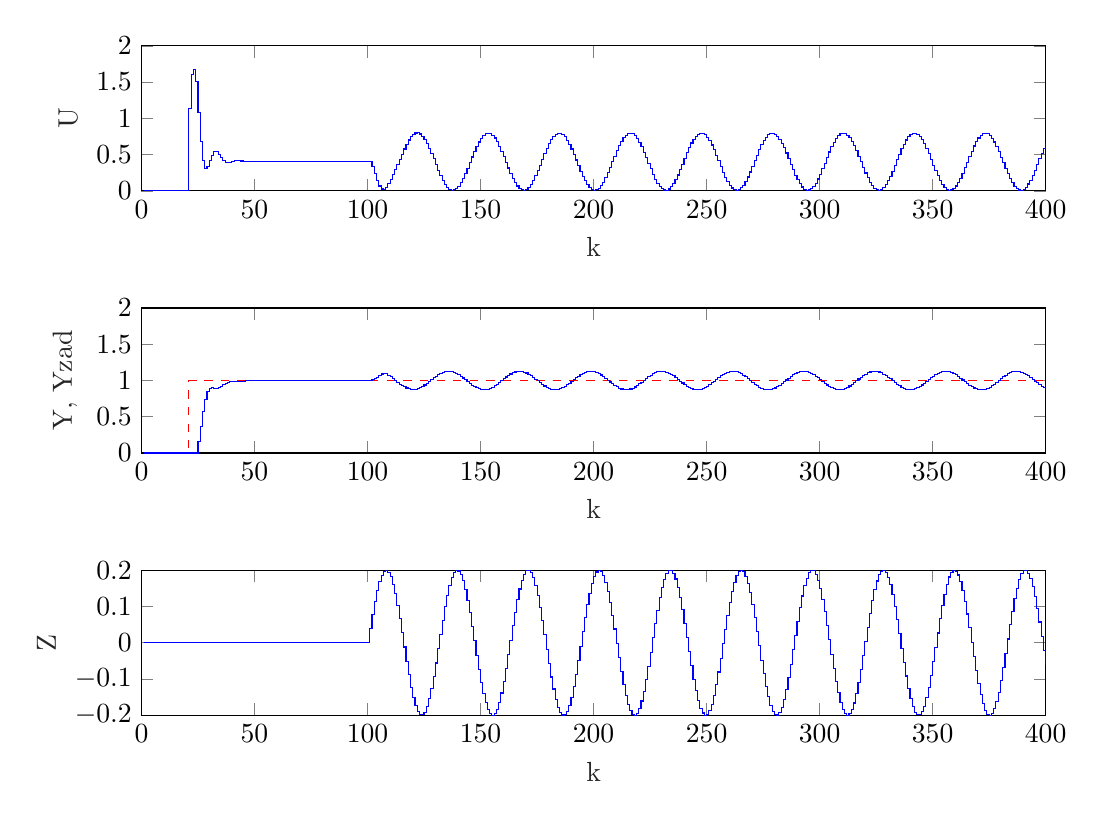
\begin{tikzpicture}

\begin{axis}[%
width=4.521in,
height=0.725in,
at={(0.758in,3.322in)},
scale only axis,
xmin=0,
xmax=400,
xlabel style={font=\color{white!15!black}},
xlabel={k},
ymin=0,
ymax=2,
ylabel style={font=\color{white!15!black}},
ylabel={U},
axis background/.style={fill=white}
]
\addplot[const plot, color=blue, forget plot] table[row sep=crcr] {%
1	0\\
2	0\\
3	0\\
4	0\\
5	0\\
6	0\\
7	0\\
8	0\\
9	0\\
10	0\\
11	0\\
12	0\\
13	0\\
14	0\\
15	0\\
16	0\\
17	0\\
18	0\\
19	0\\
20	0\\
21	1.13124041331753\\
22	1.60739620208848\\
23	1.67029772812697\\
24	1.5088290696095\\
25	1.08258009935487\\
26	0.684037120257817\\
27	0.424015380122655\\
28	0.310055013493176\\
29	0.329911659559614\\
30	0.412055543717462\\
31	0.49284813281035\\
32	0.53826796688865\\
33	0.537912993315766\\
34	0.504308140292631\\
35	0.45877281065022\\
36	0.419410565589577\\
37	0.396275443971251\\
38	0.390196587205243\\
39	0.395737940223536\\
40	0.405530115035693\\
41	0.413556147410279\\
42	0.416831988264799\\
43	0.415363749413303\\
44	0.41100616794113\\
45	0.406084453780792\\
46	0.402349250225408\\
47	0.40052789855623\\
48	0.400422166673599\\
49	0.401311205757422\\
50	0.402400609633999\\
51	0.403135629315426\\
52	0.403312371317209\\
53	0.403020350347085\\
54	0.402499132197402\\
55	0.401993011482922\\
56	0.401657765772953\\
57	0.40153450897489\\
58	0.401575545994931\\
59	0.40169360029823\\
60	0.40180770201165\\
61	0.401870068243431\\
62	0.401871046600647\\
63	0.40182832958733\\
64	0.401770153994924\\
65	0.401720848379131\\
66	0.401693163682481\\
67	0.401687705971358\\
68	0.401697066358232\\
69	0.40171140175517\\
70	0.401722879568028\\
71	0.401727766843836\\
72	0.401726257840868\\
73	0.401720930851284\\
74	0.401714902237765\\
75	0.401710465406525\\
76	0.401708535593691\\
77	0.401708807856827\\
78	0.40171030785626\\
79	0.401711988442695\\
80	0.401713135670161\\
81	0.401713504677854\\
82	0.401713234372025\\
83	0.401712653194794\\
84	0.401712087119452\\
85	0.401711739451988\\
86	0.401711660141687\\
87	0.401711782952107\\
88	0.401711991877851\\
89	0.401712181631659\\
90	0.401712292121399\\
91	0.40171231376668\\
92	0.401712272378503\\
93	0.401712206636815\\
94	0.401712149141236\\
95	0.401712116674031\\
96	0.401712109863984\\
97	0.401712118919425\\
98	0.401712131093258\\
99	0.401712136499113\\
100	0.401712130744792\\
101	0.401712114581669\\
102	0.334235295364013\\
103	0.2390343889258\\
104	0.143935098022229\\
105	0.0662976248260884\\
106	0.0255747278831896\\
107	0.0227085536006074\\
108	0.0503631547944995\\
109	0.0991979273976707\\
110	0.159444836804326\\
111	0.224891277756517\\
112	0.292813223027465\\
113	0.362441718882142\\
114	0.433642449231152\\
115	0.505562759706866\\
116	0.576108472576573\\
117	0.642174627887164\\
118	0.700215593912494\\
119	0.746920992479067\\
120	0.779723885135827\\
121	0.797031795494936\\
122	0.798224823517292\\
123	0.783510614938869\\
124	0.753742233375495\\
125	0.710272563829294\\
126	0.654867854582507\\
127	0.58966678082823\\
128	0.517152990292335\\
129	0.440110251554892\\
130	0.361543366322557\\
131	0.28456433264335\\
132	0.212255505643744\\
133	0.147526709075593\\
134	0.0929819233198008\\
135	0.0508061733855565\\
136	0.0226775599909048\\
137	0.00970511872147983\\
138	0.0123911417639461\\
139	0.0306163846595809\\
140	0.0636472807968308\\
141	0.110164968976698\\
142	0.168316022288995\\
143	0.235784119868662\\
144	0.309880741948237\\
145	0.387651658828556\\
146	0.465994863480688\\
147	0.541784868581303\\
148	0.611998000911901\\
149	0.673833415763506\\
150	0.724824910136951\\
151	0.76293913322666\\
152	0.786656411048066\\
153	0.795031094710474\\
154	0.787729109409936\\
155	0.765041228752116\\
156	0.727871519925772\\
157	0.677701374692524\\
158	0.6165305182971\\
159	0.546797323987093\\
160	0.47128160592513\\
161	0.392993775971781\\
162	0.315054798670057\\
163	0.240571743255718\\
164	0.172513900767026\\
165	0.113594405337491\\
166	0.0661620751216979\\
167	0.0321077796568143\\
168	0.0127890624508853\\
169	0.00897602199317402\\
170	0.020820608935247\\
171	0.0478505648888333\\
172	0.088988246151833\\
173	0.14259358312961\\
174	0.206529463264589\\
175	0.278246930688012\\
176	0.354886805430513\\
177	0.433393670401413\\
178	0.510637681463889\\
179	0.583539344299978\\
180	0.649192283683627\\
181	0.704979110913078\\
182	0.748675770303983\\
183	0.778540204881413\\
184	0.793381806471504\\
185	0.792608881398111\\
186	0.776252239413078\\
187	0.744963965386782\\
188	0.699991422695134\\
189	0.643127524700198\\
190	0.576639256856359\\
191	0.503177299059485\\
192	0.425670351326792\\
193	0.347208375716671\\
194	0.270919409263848\\
195	0.19984485900324\\
196	0.136818250668902\\
197	0.0843522649689548\\
198	0.0445385649409795\\
199	0.0189644079550476\\
200	0.00864936678234701\\
201	0.0140046824626434\\
202	0.0348168694448468\\
203	0.0702562266124021\\
204	0.118909914885383\\
205	0.178838282698892\\
206	0.247652193837894\\
207	0.32260827481125\\
208	0.400718284552564\\
209	0.478868246223199\\
210	0.553942591708697\\
211	0.622948369559626\\
212	0.683134564598481\\
213	0.732101772296593\\
214	0.767897855549882\\
215	0.789095770319742\\
216	0.794850457476509\\
217	0.784932513000496\\
218	0.759737271286672\\
219	0.720268949246041\\
220	0.668100859560196\\
221	0.605312757395917\\
222	0.534407921097868\\
223	0.458210510739775\\
224	0.379758991886682\\
225	0.302182596493468\\
226	0.228575357740125\\
227	0.161873214520335\\
228	0.104735471037573\\
229	0.0594390395911265\\
230	0.0277884046652801\\
231	0.0110440870673605\\
232	0.00987295215752237\\
233	0.0243217517293651\\
234	0.0538150234321128\\
235	0.0971777140479765\\
236	0.152681693225108\\
237	0.218114461841866\\
238	0.290867358364439\\
239	0.368039678694765\\
240	0.446554485881807\\
241	0.523281414217985\\
242	0.595161526893795\\
243	0.659329251313597\\
244	0.713226558419802\\
245	0.754704871631463\\
246	0.782110672883595\\
247	0.794351405534735\\
248	0.790939043088506\\
249	0.772009573099859\\
250	0.738317604062009\\
251	0.691206299608933\\
252	0.632553835215928\\
253	0.564698514765994\\
254	0.490345538308765\\
255	0.412459143759277\\
256	0.334144426120043\\
257	0.258523546460307\\
258	0.188611264335441\\
259	0.127194753366711\\
260	0.0767224892180033\\
261	0.0392066384976454\\
262	0.0161428399609795\\
263	0.00845057676541253\\
264	0.0164365178775388\\
265	0.0397822908440518\\
266	0.0775571737384079\\
267	0.128255200251305\\
268	0.189855198372299\\
269	0.259901368764616\\
270	0.335601190173868\\
271	0.413936748591808\\
272	0.4917850518725\\
273	0.566042533353708\\
274	0.633748781041464\\
275	0.69220455974909\\
276	0.739079421045906\\
277	0.77250461092451\\
278	0.79114757120594\\
279	0.794265064503145\\
280	0.781732804791574\\
281	0.75405041230407\\
282	0.712321495224436\\
283	0.658209652276577\\
284	0.593872150262119\\
285	0.521873920621949\\
286	0.445085303708022\\
287	0.366567617374191\\
288	0.289451111899039\\
289	0.216810176787778\\
290	0.151540774561792\\
291	0.0962449878640206\\
292	0.0531272826245305\\
293	0.0239066229486957\\
294	0.00974794143166188\\
295	0.0112156969620783\\
296	0.0282513715186682\\
297	0.0601758030966688\\
298	0.105716262945111\\
299	0.163057200168537\\
300	0.229912632429163\\
301	0.303617276120156\\
302	0.381232793290691\\
303	0.459664925247105\\
304	0.535787009633834\\
305	0.606564431000964\\
306	0.669175540633437\\
307	0.721124161112345\\
308	0.760339093189237\\
309	0.785256773125997\\
310	0.794883679886671\\
311	0.788835972179991\\
312	0.767354792390088\\
313	0.731296617089881\\
314	0.682099065180771\\
315	0.621723550302131\\
316	0.55257707060558\\
317	0.477416255926487\\
318	0.39923748936748\\
319	0.32115747209571\\
320	0.246288984790514\\
321	0.177616795072957\\
322	0.11787865947241\\
323	0.0694561685167154\\
324	0.034279791350528\\
325	0.013751908682509\\
326	0.00869090341773893\\
327	0.0192985368458738\\
328	0.0451519089936488\\
329	0.085220321754142\\
330	0.13790637139168\\
331	0.201109632034122\\
332	0.272310391846315\\
333	0.348670104419918\\
334	0.427144551410107\\
335	0.504605205343635\\
336	0.57796395423722\\
337	0.644296215393767\\
338	0.700957529891402\\
339	0.745688989258491\\
340	0.776707291196853\\
341	0.792775834143517\\
342	0.793254016464086\\
343	0.778122774997156\\
344	0.747985344894957\\
345	0.704043210497858\\
346	0.648048205987048\\
347	0.582232675367318\\
348	0.509220476036542\\
349	0.431922373920278\\
350	0.353420000430134\\
351	0.276842997525196\\
352	0.20524424873227\\
353	0.141478170286089\\
354	0.0880869145467008\\
355	0.0471990224060222\\
356	0.0204445650879757\\
357	0.00889015836454157\\
358	0.0129964399604433\\
359	0.0325997053853986\\
360	0.0669184343153632\\
361	0.114584447338314\\
362	0.173697450945774\\
363	0.241900796235197\\
364	0.316475431063621\\
365	0.394448300076565\\
366	0.472710871044376\\
367	0.548143062234197\\
368	0.617737630223725\\
369	0.678720059206948\\
370	0.728659172183642\\
371	0.765564054313876\\
372	0.78796342440949\\
373	0.794964290271864\\
374	0.786287549472819\\
375	0.762279116287779\\
376	0.723896131185407\\
377	0.672668802657736\\
378	0.610639402636554\\
379	0.540280847556268\\
380	0.46439811097937\\
381	0.386016398152041\\
382	0.308260540617524\\
383	0.234230419043448\\
384	0.166877380761845\\
385	0.108886578864567\\
386	0.0625699236230218\\
387	0.0297739139213382\\
388	0.0118060231728269\\
389	0.00938257448095886\\
390	0.0226001830977192\\
391	0.050931904678384\\
392	0.0932482428896748\\
393	0.14786217886423\\
394	0.212596427319152\\
395	0.284870238049415\\
396	0.36180228229452\\
397	0.44032552222361\\
398	0.51730948405519\\
399	0.589685060168019\\
400	0.654566864736822\\
};
\end{axis}

\begin{axis}[%
width=4.521in,
height=0.725in,
at={(0.758in,2.011in)},
scale only axis,
xmin=0,
xmax=400,
xlabel style={font=\color{white!15!black}},
xlabel={k},
ymin=0,
ymax=2,
ylabel style={font=\color{white!15!black}},
ylabel={Y, Yzad},
axis background/.style={fill=white}
]
\addplot[const plot, color=red, dashed, forget plot] table[row sep=crcr] {%
1	0\\
2	0\\
3	0\\
4	0\\
5	0\\
6	0\\
7	0\\
8	0\\
9	0\\
10	0\\
11	0\\
12	0\\
13	0\\
14	0\\
15	0\\
16	0\\
17	0\\
18	0\\
19	0\\
20	0\\
21	1\\
22	1\\
23	1\\
24	1\\
25	1\\
26	1\\
27	1\\
28	1\\
29	1\\
30	1\\
31	1\\
32	1\\
33	1\\
34	1\\
35	1\\
36	1\\
37	1\\
38	1\\
39	1\\
40	1\\
41	1\\
42	1\\
43	1\\
44	1\\
45	1\\
46	1\\
47	1\\
48	1\\
49	1\\
50	1\\
51	1\\
52	1\\
53	1\\
54	1\\
55	1\\
56	1\\
57	1\\
58	1\\
59	1\\
60	1\\
61	1\\
62	1\\
63	1\\
64	1\\
65	1\\
66	1\\
67	1\\
68	1\\
69	1\\
70	1\\
71	1\\
72	1\\
73	1\\
74	1\\
75	1\\
76	1\\
77	1\\
78	1\\
79	1\\
80	1\\
81	1\\
82	1\\
83	1\\
84	1\\
85	1\\
86	1\\
87	1\\
88	1\\
89	1\\
90	1\\
91	1\\
92	1\\
93	1\\
94	1\\
95	1\\
96	1\\
97	1\\
98	1\\
99	1\\
100	1\\
101	1\\
102	1\\
103	1\\
104	1\\
105	1\\
106	1\\
107	1\\
108	1\\
109	1\\
110	1\\
111	1\\
112	1\\
113	1\\
114	1\\
115	1\\
116	1\\
117	1\\
118	1\\
119	1\\
120	1\\
121	1\\
122	1\\
123	1\\
124	1\\
125	1\\
126	1\\
127	1\\
128	1\\
129	1\\
130	1\\
131	1\\
132	1\\
133	1\\
134	1\\
135	1\\
136	1\\
137	1\\
138	1\\
139	1\\
140	1\\
141	1\\
142	1\\
143	1\\
144	1\\
145	1\\
146	1\\
147	1\\
148	1\\
149	1\\
150	1\\
151	1\\
152	1\\
153	1\\
154	1\\
155	1\\
156	1\\
157	1\\
158	1\\
159	1\\
160	1\\
161	1\\
162	1\\
163	1\\
164	1\\
165	1\\
166	1\\
167	1\\
168	1\\
169	1\\
170	1\\
171	1\\
172	1\\
173	1\\
174	1\\
175	1\\
176	1\\
177	1\\
178	1\\
179	1\\
180	1\\
181	1\\
182	1\\
183	1\\
184	1\\
185	1\\
186	1\\
187	1\\
188	1\\
189	1\\
190	1\\
191	1\\
192	1\\
193	1\\
194	1\\
195	1\\
196	1\\
197	1\\
198	1\\
199	1\\
200	1\\
201	1\\
202	1\\
203	1\\
204	1\\
205	1\\
206	1\\
207	1\\
208	1\\
209	1\\
210	1\\
211	1\\
212	1\\
213	1\\
214	1\\
215	1\\
216	1\\
217	1\\
218	1\\
219	1\\
220	1\\
221	1\\
222	1\\
223	1\\
224	1\\
225	1\\
226	1\\
227	1\\
228	1\\
229	1\\
230	1\\
231	1\\
232	1\\
233	1\\
234	1\\
235	1\\
236	1\\
237	1\\
238	1\\
239	1\\
240	1\\
241	1\\
242	1\\
243	1\\
244	1\\
245	1\\
246	1\\
247	1\\
248	1\\
249	1\\
250	1\\
251	1\\
252	1\\
253	1\\
254	1\\
255	1\\
256	1\\
257	1\\
258	1\\
259	1\\
260	1\\
261	1\\
262	1\\
263	1\\
264	1\\
265	1\\
266	1\\
267	1\\
268	1\\
269	1\\
270	1\\
271	1\\
272	1\\
273	1\\
274	1\\
275	1\\
276	1\\
277	1\\
278	1\\
279	1\\
280	1\\
281	1\\
282	1\\
283	1\\
284	1\\
285	1\\
286	1\\
287	1\\
288	1\\
289	1\\
290	1\\
291	1\\
292	1\\
293	1\\
294	1\\
295	1\\
296	1\\
297	1\\
298	1\\
299	1\\
300	1\\
301	1\\
302	1\\
303	1\\
304	1\\
305	1\\
306	1\\
307	1\\
308	1\\
309	1\\
310	1\\
311	1\\
312	1\\
313	1\\
314	1\\
315	1\\
316	1\\
317	1\\
318	1\\
319	1\\
320	1\\
321	1\\
322	1\\
323	1\\
324	1\\
325	1\\
326	1\\
327	1\\
328	1\\
329	1\\
330	1\\
331	1\\
332	1\\
333	1\\
334	1\\
335	1\\
336	1\\
337	1\\
338	1\\
339	1\\
340	1\\
341	1\\
342	1\\
343	1\\
344	1\\
345	1\\
346	1\\
347	1\\
348	1\\
349	1\\
350	1\\
351	1\\
352	1\\
353	1\\
354	1\\
355	1\\
356	1\\
357	1\\
358	1\\
359	1\\
360	1\\
361	1\\
362	1\\
363	1\\
364	1\\
365	1\\
366	1\\
367	1\\
368	1\\
369	1\\
370	1\\
371	1\\
372	1\\
373	1\\
374	1\\
375	1\\
376	1\\
377	1\\
378	1\\
379	1\\
380	1\\
381	1\\
382	1\\
383	1\\
384	1\\
385	1\\
386	1\\
387	1\\
388	1\\
389	1\\
390	1\\
391	1\\
392	1\\
393	1\\
394	1\\
395	1\\
396	1\\
397	1\\
398	1\\
399	1\\
400	1\\
};
\addplot[const plot, color=blue, forget plot] table[row sep=crcr] {%
1	0\\
2	0\\
3	0\\
4	0\\
5	0\\
6	0\\
7	0\\
8	0\\
9	0\\
10	0\\
11	0\\
12	0\\
13	0\\
14	0\\
15	0\\
16	0\\
17	0\\
18	0\\
19	0\\
20	0\\
21	0\\
22	0\\
23	0\\
24	0\\
25	0.152830579839198\\
26	0.361723685979986\\
27	0.567813252929803\\
28	0.740934525440941\\
29	0.847095360437015\\
30	0.893658115143514\\
31	0.90255973864811\\
32	0.895570671873684\\
33	0.89163036498361\\
34	0.898990405246294\\
35	0.91685828271975\\
36	0.939887677878803\\
37	0.961615803129477\\
38	0.977621370527924\\
39	0.986602460199098\\
40	0.989773437013205\\
41	0.989641380644215\\
42	0.988689847199495\\
43	0.988533654813312\\
44	0.989704626042417\\
45	0.991892848316057\\
46	0.994401945347177\\
47	0.996573965969035\\
48	0.998037076898529\\
49	0.998753666950623\\
50	0.998924656597726\\
51	0.998838350857697\\
52	0.998740665168325\\
53	0.998766808279368\\
54	0.998937329483177\\
55	0.999196697549384\\
56	0.999464818354491\\
57	0.999678006297738\\
58	0.999808372281484\\
59	0.999862529279366\\
60	0.999867769339971\\
61	0.999855454910885\\
62	0.999848800913543\\
63	0.999857968169211\\
64	0.999881621834702\\
65	0.999912037309881\\
66	0.999940598025195\\
67	0.999961538784302\\
68	0.999973216807206\\
69	0.999977361349574\\
70	0.999977327623101\\
71	0.999976368399375\\
72	0.999976556980123\\
73	0.999978522354457\\
74	0.999981799158156\\
75	0.999985440953475\\
76	0.999988577040411\\
77	0.999990730653257\\
78	0.99999187053213\\
79	0.999992275801492\\
80	0.999992333120867\\
81	0.99999236613075\\
82	0.999992548519416\\
83	0.999992902381439\\
84	0.999993351510946\\
85	0.999993790164412\\
86	0.999994136571704\\
87	0.999994357305398\\
88	0.999994464385011\\
89	0.999994496292151\\
90	0.999994495860299\\
91	0.999994494377281\\
92	0.999994505516522\\
93	0.999994527765157\\
94	0.999994551375948\\
95	0.999994565659013\\
96	0.999994563834085\\
97	0.999994544575335\\
98	0.999994510910527\\
99	0.999994467862375\\
100	0.999994420170427\\
101	0.999994370909295\\
102	1.00846756814737\\
103	1.02412524042148\\
104	1.04549873740651\\
105	1.07098615417743\\
106	1.0897894869801\\
107	1.09695204608207\\
108	1.09148974686446\\
109	1.07482345376639\\
110	1.05099280528335\\
111	1.0240726379727\\
112	0.997106822830562\\
113	0.971940429321492\\
114	0.949265271494161\\
115	0.929190730356925\\
116	0.911763172898169\\
117	0.897237902125641\\
118	0.886145599729037\\
119	0.879160275186301\\
120	0.876892346374106\\
121	0.879713998401527\\
122	0.887662570353424\\
123	0.900434028800379\\
124	0.917441234462095\\
125	0.937898460658789\\
126	0.960901757791112\\
127	0.98548850360104\\
128	1.0106745836872\\
129	1.03547746195109\\
130	1.05893570747977\\
131	1.08013275997311\\
132	1.09822753530338\\
133	1.11248968877153\\
134	1.12233470367997\\
135	1.12735367004439\\
136	1.12733400610924\\
137	1.1222694285396\\
138	1.11235929446379\\
139	1.09799855160112\\
140	1.07975990052392\\
141	1.05836963742826\\
142	1.0346783377447\\
143	1.00962731998219\\
144	0.984211811732718\\
145	0.959441906336624\\
146	0.936302648672162\\
147	0.915714805896407\\
148	0.898497980345131\\
149	0.885337675649939\\
150	0.876757747820665\\
151	0.87309940097526\\
152	0.87450756758343\\
153	0.880925180462769\\
154	0.892095518043524\\
155	0.907572492709888\\
156	0.926738455234154\\
157	0.948828807409089\\
158	0.972962454691947\\
159	0.998176900080328\\
160	1.02346659118666\\
161	1.04782299602912\\
162	1.07027480826367\\
163	1.0899266742636\\
164	1.10599489310515\\
165	1.11783866284971\\
166	1.12498562633376\\
167	1.12715069876355\\
168	1.12424742812056\\
169	1.11639143703251\\
170	1.10389580984113\\
171	1.08725860897402\\
172	1.06714301795446\\
173	1.04435090210635\\
174	1.01979084048842\\
175	0.994441903229234\\
176	0.969314618296533\\
177	0.945410683951149\\
178	0.923683033200544\\
179	0.90499784250252\\
180	0.890099999381749\\
181	0.879583405648838\\
182	0.873867300082941\\
183	0.87317954444952\\
184	0.877547539133908\\
185	0.886797130530064\\
186	0.900559553743016\\
187	0.918286133835661\\
188	0.939270159544737\\
189	0.962675057441526\\
190	0.987567743325218\\
191	1.01295582122954\\
192	1.03782714702727\\
193	1.06119017934828\\
194	1.08211350914147\\
195	1.09976299195905\\
196	1.11343500261617\\
197	1.12258448646869\\
198	1.12684668899436\\
199	1.12605169738803\\
200	1.12023121444303\\
201	1.10961729466431\\
202	1.09463309299939\\
203	1.07587599500484\\
204	1.05409380099472\\
205	1.03015491363343\\
206	1.00501371749964\\
207	0.979672530828834\\
208	0.955141646298545\\
209	0.93239905390413\\
210	0.912351451646891\\
211	0.89579809841531\\
212	0.883398950130936\\
213	0.875648349470253\\
214	0.872855318070408\\
215	0.8751312369065\\
216	0.882385405985153\\
217	0.894328660375589\\
218	0.910484898418745\\
219	0.930210062521374\\
220	0.952717815831076\\
221	0.977110888476762\\
222	1.00241683807791\\
223	1.02762679487319\\
224	1.05173569387671\\
225	1.07378236413806\\
226	1.09288786616339\\
227	1.10829016584793\\
228	1.11937498009483\\
229	1.12570038196096\\
230	1.1270143644332\\
231	1.12326489694906\\
232	1.11460180714353\\
233	1.10137066079897\\
234	1.08409894590141\\
235	1.06347506064144\\
236	1.04032096132319\\
237	1.01555949800297\\
238	0.990177690182373\\
239	0.965187397611719\\
240	0.941584954854863\\
241	0.920311400957579\\
242	0.902214916390749\\
243	0.888016980815316\\
244	0.878283606190112\\
245	0.87340278650983\\
246	0.873569051841418\\
247	0.878775731955199\\
248	0.888815231775185\\
249	0.90328730687906\\
250	0.921615012474442\\
251	0.943067694883721\\
252	0.966790113042385\\
253	0.991836531061098\\
254	1.01720842252499\\
255	1.04189428178203\\
256	1.06490995309411\\
257	1.08533786835933\\
258	1.10236362851188\\
259	1.11530847043164\\
260	1.12365632570349\\
261	1.12707439323494\\
262	1.12542640608237\\
263	1.11877806374181\\
264	1.10739441320076\\
265	1.09172928287598\\
266	1.07240719039432\\
267	1.05019844532511\\
268	1.02598843940275\\
269	1.00074234860858\\
270	0.975466654438754\\
271	0.951169018482647\\
272	0.92881811003964\\
273	0.909304988325098\\
274	0.893407578805095\\
275	0.88175965983456\\
276	0.874825595969611\\
277	0.872881825240674\\
278	0.876005838431606\\
279	0.884073089738624\\
280	0.896761961986487\\
281	0.913566588465848\\
282	0.933817020230242\\
283	0.956705934844739\\
284	0.981320821787769\\
285	1.00668036137025\\
286	1.03177354685556\\
287	1.05559999010362\\
288	1.07720980388108\\
289	1.09574147085762\\
290	1.11045618957281\\
291	1.12076732810955\\
292	1.12626381124908\\
293	1.12672650873526\\
294	1.12213697129903\\
295	1.11267816616442\\
296	1.09872718271368\\
297	1.08084019911341\\
298	1.05973030923506\\
299	1.0362390938407\\
300	1.01130306940141\\
301	0.985916352128886\\
302	0.961091025848729\\
303	0.937816794218676\\
304	0.917021526537232\\
305	0.899534267936835\\
306	0.886052188021748\\
307	0.877112785794239\\
308	0.873072481651674\\
309	0.874092400348387\\
310	0.880131931991292\\
311	0.890950338331847\\
312	0.906116337171324\\
313	0.925025295364656\\
314	0.946923342667026\\
315	0.970937438554292\\
316	0.996110189504144\\
317	1.02143802367071\\
318	1.04591119986754\\
319	1.06855405788774\\
320	1.08846390837952\\
321	1.10484701485248\\
322	1.11705023503116\\
323	1.12458706014706\\
324	1.12715701300522\\
325	1.12465762998774\\
326	1.11718854807855\\
327	1.10504753341758\\
328	1.08871860982925\\
329	1.06885276114891\\
330	1.04624197732578\\
331	1.02178767946545\\
332	0.996464782773813\\
333	0.971282830001139\\
334	0.947245744628957\\
335	0.925311808060194\\
336	0.906355456231456\\
337	0.891132418652912\\
338	0.880249589727547\\
339	0.874140833586369\\
340	0.873049687118955\\
341	0.87701965082978\\
342	0.885892454601059\\
343	0.899314367473909\\
344	0.916750299856761\\
345	0.937505135916384\\
346	0.960751445678871\\
347	0.985562472046567\\
348	1.01094907765433\\
349	1.03589917862562\\
350	1.05941809314088\\
351	1.08056819625322\\
352	1.098506300038\\
353	1.11251726884294\\
354	1.12204252949913\\
355	1.12670233987682\\
356	1.12631092800755\\
357	1.12088389822417\\
358	1.11063760906137\\
359	1.09598054771972\\
360	1.07749704496748\\
361	1.05592397971601\\
362	1.03212140198339\\
363	1.00703824541545\\
364	0.981674496296792\\
365	0.957041327253833\\
366	0.934120784993076\\
367	0.913826639197481\\
368	0.896967953412166\\
369	0.884216830233491\\
370	0.876081616699184\\
371	0.872886638096041\\
372	0.874759268134281\\
373	0.881624850959779\\
374	0.893209677447466\\
375	0.909051897120418\\
376	0.928519930670865\\
377	0.950837649034038\\
378	0.975115315204665\\
379	1.00038505524357\\
380	1.02563944435729\\
381	1.04987166974545\\
382	1.07211566904993\\
383	1.09148464421251\\
384	1.107206415315\\
385	1.11865420495579\\
386	1.12537162588696\\
387	1.12709087573358\\
388	1.12374341342932\\
389	1.11546269173243\\
390	1.10257883688542\\
391	1.0856054875235\\
392	1.06521931752312\\
393	1.04223305914983\\
394	1.01756310198761\\
395	0.992192959377957\\
396	0.967134058846649\\
397	0.943385419679988\\
398	0.921893825178462\\
399	0.903516077394291\\
400	0.888984839137397\\
};
\end{axis}

\begin{axis}[%
width=4.521in,
height=0.725in,
at={(0.758in,0.7in)},
scale only axis,
xmin=0,
xmax=400,
xlabel style={font=\color{white!15!black}},
xlabel={k},
ymin=-0.2,
ymax=0.2,
ylabel style={font=\color{white!15!black}},
ylabel={Z},
axis background/.style={fill=white}
]
\addplot[const plot, color=blue, forget plot] table[row sep=crcr] {%
1	0\\
2	0\\
3	0\\
4	0\\
5	0\\
6	0\\
7	0\\
8	0\\
9	0\\
10	0\\
11	0\\
12	0\\
13	0\\
14	0\\
15	0\\
16	0\\
17	0\\
18	0\\
19	0\\
20	0\\
21	0\\
22	0\\
23	0\\
24	0\\
25	0\\
26	0\\
27	0\\
28	0\\
29	0\\
30	0\\
31	0\\
32	0\\
33	0\\
34	0\\
35	0\\
36	0\\
37	0\\
38	0\\
39	0\\
40	0\\
41	0\\
42	0\\
43	0\\
44	0\\
45	0\\
46	0\\
47	0\\
48	0\\
49	0\\
50	0\\
51	0\\
52	0\\
53	0\\
54	0\\
55	0\\
56	0\\
57	0\\
58	0\\
59	0\\
60	0\\
61	0\\
62	0\\
63	0\\
64	0\\
65	0\\
66	0\\
67	0\\
68	0\\
69	0\\
70	0\\
71	0\\
72	0\\
73	0\\
74	0\\
75	0\\
76	0\\
77	0\\
78	0\\
79	0\\
80	0\\
81	0\\
82	0\\
83	0\\
84	0\\
85	0\\
86	0\\
87	0\\
88	0\\
89	0\\
90	0\\
91	0\\
92	0\\
93	0\\
94	0\\
95	0\\
96	0\\
97	0\\
98	0\\
99	0\\
100	0\\
101	0.0397338661590122\\
102	0.0778836684617301\\
103	0.112928494679007\\
104	0.143471218179905\\
105	0.168294196961579\\
106	0.186407817193445\\
107	0.197089945997692\\
108	0.199914720608301\\
109	0.194769526175639\\
110	0.181859485365136\\
111	0.161699280763918\\
112	0.13509263611023\\
113	0.103100274364293\\
114	0.0669976300311809\\
115	0.0282240016119734\\
116	-0.011674828685516\\
117	-0.0511082204053663\\
118	-0.0885040886589705\\
119	-0.122371578188544\\
120	-0.151360499061586\\
121	-0.174315154482718\\
122	-0.190320414777903\\
123	-0.198738200726693\\
124	-0.199232921767168\\
125	-0.191784854932628\\
126	-0.176690931144031\\
127	-0.154552897511197\\
128	-0.126253327574464\\
129	-0.0929204358827513\\
130	-0.0558830996397852\\
131	-0.0166178805634993\\
132	0.0233098409700987\\
133	0.0623082727026757\\
134	0.0988226702277218\\
135	0.131397319743758\\
136	0.158733572769831\\
137	0.179741619162325\\
138	0.193583934406297\\
139	0.199708669074921\\
140	0.197871649324676\\
141	0.188146111335955\\
142	0.170919781617656\\
143	0.146879419574823\\
144	0.116983438578352\\
145	0.0824236970483513\\
146	0.0445779828200492\\
147	0.00495508509067155\\
148	-0.0348653562445963\\
149	-0.0732958258503857\\
150	-0.108804222177874\\
151	-0.139974937518709\\
152	-0.165565293817131\\
153	-0.184555084322561\\
154	-0.196187246013298\\
155	-0.199998041310141\\
156	-0.195835545830263\\
157	-0.183865705132935\\
158	-0.164565718993742\\
159	-0.138705016955424\\
160	-0.107314583600087\\
161	-0.0716458564473654\\
162	-0.0331208350896619\\
163	0.00672460944422769\\
164	0.0463019650203078\\
165	0.0840334073653282\\
166	0.118414702941445\\
167	0.14807517799049\\
168	0.171832362971299\\
169	0.188739133888821\\
170	0.198121471138974\\
171	0.199605330543272\\
172	0.193131555309855\\
173	0.178958234428101\\
174	0.157650413475063\\
175	0.130057568031423\\
176	0.0972797377707596\\
177	0.0606236713491405\\
178	0.0215507304598885\\
179	-0.0183813700455363\\
180	-0.0575806633330131\\
181	-0.0944843972796932\\
182	-0.12762133646959\\
183	-0.15567041570686\\
184	-0.177513406716301\\
185	-0.192279498375911\\
186	-0.199380013208319\\
187	-0.198531876094127\\
188	-0.189768899583625\\
189	-0.173440435897116\\
190	-0.150197449354335\\
191	-0.120966564481257\\
192	-0.0869131244143787\\
193	-0.0493947323473242\\
194	-0.00990712817567348\\
195	0.0299754419325905\\
196	0.0686629857639798\\
197	0.10461315303154\\
198	0.136392724013627\\
199	0.162734747501421\\
200	0.182589050145526\\
201	0.195164103553395\\
202	0.199958580028534\\
203	0.196781338923723\\
204	0.185759046815448\\
205	0.167331127707211\\
206	0.142232244581196\\
207	0.111463010703532\\
208	0.076250098330988\\
209	0.0379973351590875\\
210	-0.00177026185808078\\
211	-0.0414672841213524\\
212	-0.0795111366242872\\
213	-0.114385131021913\\
214	-0.144698951208849\\
215	-0.169244080835034\\
216	-0.187041983038908\\
217	-0.19738311162413\\
218	-0.199855198427326\\
219	-0.194359689148773\\
220	-0.181115672401325\\
221	-0.160651145338791\\
222	-0.133781964075604\\
223	-0.101579318078124\\
224	-0.0653270252209445\\
225	-0.0264703500195546\\
226	0.0134416145050957\\
227	0.0528177042768946\\
228	0.0900881188550779\\
229	0.123767004424008\\
230	0.152511690095921\\
231	0.175176215962178\\
232	0.19085701889854\\
233	0.198928954775568\\
234	0.199070220982312\\
235	0.191275185680901\\
236	0.175854612330145\\
237	0.153423270527106\\
238	0.124875427083278\\
239	0.0913491944288386\\
240	0.0541811576615738\\
241	0.0148530891168716\\
242	-0.0250671252192865\\
243	-0.0639879923768396\\
244	-0.100357860204115\\
245	-0.132726776842594\\
246	-0.159804295731923\\
247	-0.180510921642037\\
248	-0.194021146741437\\
249	-0.19979636098939\\
250	-0.197606324818572\\
251	-0.187538348060056\\
252	-0.169993809175866\\
253	-0.145672153566319\\
254	-0.115543008889147\\
255	-0.080807529064613\\
256	-0.0428505080591775\\
257	-0.00318517252002036\\
258	0.0366071457961169\\
259	0.0749400527298918\\
260	0.110285336248338\\
261	0.141233891436067\\
262	0.166551897061556\\
263	0.185230004136105\\
264	0.196523575472828\\
265	0.199982372021453\\
266	0.195468502478452\\
267	0.183161920578164\\
268	0.163553250905289\\
269	0.137424229240949\\
270	0.105816537224005\\
271	0.0699902737913324\\
272	0.031373719009682\\
273	-0.00849360694338889\\
274	-0.0480223195907549\\
275	-0.0856365338992302\\
276	-0.119836689842853\\
277	-0.149259335128983\\
278	-0.17273148173859\\
279	-0.189317369256992\\
280	-0.198355770688623\\
281	-0.19948635349073\\
282	-0.192664044894752\\
283	-0.178160828815373\\
284	-0.156554902710131\\
285	-0.1287076266714\\
286	-0.095729183717683\\
287	-0.0589343203000515\\
288	-0.0197899315100593\\
289	0.0201434193985001\\
290	0.0592737157418771\\
291	0.0960409560876518\\
292	0.128979346588973\\
293	0.156775737559658\\
294	0.178321974608288\\
295	0.192759077256818\\
296	0.199511483781561\\
297	0.198309997042828\\
298	0.189202516525382\\
299	0.172552128737136\\
300	0.14902263209587\\
301	0.119552073381051\\
302	0.0853153507689146\\
303	0.0476773743497798\\
304	0.00813865146997297\\
305	-0.0317245337609418\\
306	-0.0703229619433633\\
307	-0.106117835550041\\
308	-0.137682125927533\\
309	-0.163757464425369\\
310	-0.183304309583127\\
311	-0.195543390368004\\
312	-0.199986773251761\\
313	-0.196457314580727\\
314	-0.185095722734266\\
315	-0.16635494852572\\
316	-0.14098212748285\\
317	-0.10998879391207\\
318	-0.0746105542177258\\
319	-0.036257827173939\\
320	0.00354038502108272\\
321	0.0431974532376448\\
322	0.0811323753110672\\
323	0.115832805608854\\
324	0.145915347478571\\
325	0.170180704906824\\
326	0.187661494666711\\
327	0.197660812834327\\
328	0.199780018149004\\
329	0.193934624582384\\
330	0.180357669529762\\
331	0.159590423344526\\
332	0.132460810597249\\
333	0.100050403335717\\
334	0.0636513022204976\\
335	0.0247146245490448\\
336	-0.0152073472116707\\
337	-0.0545230500286148\\
338	-0.0916650908983532\\
339	-0.125152733859895\\
340	-0.153650932264733\\
341	-0.176023552873732\\
342	-0.191378669904098\\
343	-0.199104123295703\\
344	-0.198891923600903\\
345	-0.190750530551894\\
346	-0.175004515797889\\
347	-0.152281623257708\\
348	-0.123487742950692\\
349	-0.0897707960203409\\
350	-0.0524749707407858\\
351	-0.0130871339721414\\
352	0.0268224455291314\\
353	0.0656626987702807\\
354	0.101885187422086\\
355	0.134045835168675\\
356	0.160862498473183\\
357	0.181266081594533\\
358	0.194443158060908\\
359	0.199868399416262\\
360	0.197325518408097\\
361	0.186915891677683\\
362	0.169054518193285\\
363	0.144453474550903\\
364	0.114093526727476\\
365	0.0791850300363668\\
366	0.0411196760805202\\
367	0.00141501039998619\\
368	-0.0383460672798732\\
369	-0.0765784082652954\\
370	-0.111757809770323\\
371	-0.142481780071971\\
372	-0.167525451429406\\
373	-0.185890411695483\\
374	-0.196844507858378\\
375	-0.199951034671724\\
376	-0.195086144714686\\
377	-0.182443785797804\\
378	-0.162527968875822\\
379	-0.136132674721426\\
380	-0.104310200417382\\
381	-0.0683292075925703\\
382	-0.0296241448863273\\
383	0.0102619389921399\\
384	0.0497389117464102\\
385	0.087232951049565\\
386	0.121249287873869\\
387	0.150431798214895\\
388	0.173617067476084\\
389	0.18988077213734\\
390	0.198574529616907\\
391	0.199351747238813\\
392	0.192181439789124\\
393	0.177349464798646\\
394	0.155447126305245\\
395	0.127347601427828\\
396	0.0941711295500773\\
397	0.0572403519113507\\
398	0.0180275820742931\\
399	-0.0219038905707402\\
400	-0.0609621242204433\\
};
\end{axis}
\end{tikzpicture}%
	\label{6zprzebieg}
\end{figure}

Ponieważ róznica pomiędzy rysunkiem \ref{6przebieg}, a rysunkiem \ref{5zprzebieg} nie jest zbyt wyraźna dla zadanej skali wykonano zestawienie wyjścia dla obydwu przebiegów (Rys. \ref{singraph})

\begin{figure}
	
	\centering
	\caption{ Przebieg symulacji algorytmu DMC dla zakłócenia zmiennego sinusoidalnie z uwzględnianiem zakłóceń }
	% This file was created by matlab2tikz.
%
%The latest updates can be retrieved from
%  http://www.mathworks.com/matlabcentral/fileexchange/22022-matlab2tikz-matlab2tikz
%where you can also make suggestions and rate matlab2tikz.
%
\definecolor{mycolor1}{rgb}{0.00000,0.44700,0.74100}%
\definecolor{mycolor2}{rgb}{0.85000,0.32500,0.09800}%
%
\begin{tikzpicture}

\begin{axis}[%
width=5.328in,
height=4.966in,
at={(0.894in,0.67in)},
scale only axis,
xmin=0,
xmax=400,
xlabel style={font=\color{white!15!black}},
xlabel={k},
ymin=0,
ymax=1.4,
ylabel style={font=\color{white!15!black}},
ylabel={$\text{Y,Y}_{\text{zad}}$},
axis background/.style={fill=white},
legend style={legend cell align=left, align=left, draw=white!15!black}
]
\addplot[const plot, color=mycolor1] table[row sep=crcr] {%
1	0\\
2	0\\
3	0\\
4	0\\
5	0\\
6	0\\
7	0\\
8	0\\
9	0\\
10	0\\
11	0\\
12	0\\
13	0\\
14	0\\
15	0\\
16	0\\
17	0\\
18	0\\
19	0\\
20	0\\
21	0\\
22	0\\
23	0\\
24	0\\
25	0.152830579839198\\
26	0.361723685979986\\
27	0.567813252929803\\
28	0.740934525440941\\
29	0.847095360437015\\
30	0.893658115143514\\
31	0.90255973864811\\
32	0.895570671873684\\
33	0.89163036498361\\
34	0.898990405246294\\
35	0.91685828271975\\
36	0.939887677878803\\
37	0.961615803129477\\
38	0.977621370527924\\
39	0.986602460199098\\
40	0.989773437013205\\
41	0.989641380644215\\
42	0.988689847199495\\
43	0.988533654813312\\
44	0.989704626042417\\
45	0.991892848316057\\
46	0.994401945347177\\
47	0.996573965969035\\
48	0.998037076898529\\
49	0.998753666950623\\
50	0.998924656597726\\
51	0.998838350857697\\
52	0.998740665168325\\
53	0.998766808279368\\
54	0.998937329483177\\
55	0.999196697549384\\
56	0.999464818354491\\
57	0.999678006297738\\
58	0.999808372281484\\
59	0.999862529279366\\
60	0.999867769339971\\
61	0.999855454910885\\
62	0.999848800913543\\
63	0.999857968169211\\
64	0.999881621834702\\
65	0.999912037309881\\
66	0.999940598025195\\
67	0.999961538784302\\
68	0.999973216807206\\
69	0.999977361349574\\
70	0.999977327623101\\
71	0.999976368399375\\
72	0.999976556980123\\
73	0.999978522354457\\
74	0.999981799158156\\
75	0.999985440953475\\
76	0.999988577040411\\
77	0.999990730653257\\
78	0.99999187053213\\
79	0.999992275801492\\
80	0.999992333120867\\
81	0.99999236613075\\
82	0.999992548519416\\
83	0.999992902381439\\
84	0.999993351510946\\
85	0.999993790164412\\
86	0.999994136571704\\
87	0.999994357305398\\
88	0.999994464385011\\
89	0.999994496292151\\
90	0.999994495860299\\
91	0.999994494377281\\
92	0.999994505516522\\
93	0.999994527765157\\
94	0.999994551375948\\
95	0.999994565659013\\
96	0.999994563834085\\
97	0.999994544575335\\
98	0.999994510910527\\
99	0.999994467862375\\
100	0.999994420170427\\
101	0.999994370909295\\
102	1.00846756814737\\
103	1.02412524042148\\
104	1.04549873740651\\
105	1.07098615417743\\
106	1.0897894869801\\
107	1.09695204608207\\
108	1.09148974686446\\
109	1.07482345376639\\
110	1.05099280528335\\
111	1.0240726379727\\
112	0.997106822830562\\
113	0.971940429321492\\
114	0.949265271494161\\
115	0.929190730356925\\
116	0.911763172898169\\
117	0.897237902125641\\
118	0.886145599729037\\
119	0.879160275186301\\
120	0.876892346374106\\
121	0.879713998401527\\
122	0.887662570353424\\
123	0.900434028800379\\
124	0.917441234462095\\
125	0.937898460658789\\
126	0.960901757791112\\
127	0.98548850360104\\
128	1.0106745836872\\
129	1.03547746195109\\
130	1.05893570747977\\
131	1.08013275997311\\
132	1.09822753530338\\
133	1.11248968877153\\
134	1.12233470367997\\
135	1.12735367004439\\
136	1.12733400610924\\
137	1.1222694285396\\
138	1.11235929446379\\
139	1.09799855160112\\
140	1.07975990052392\\
141	1.05836963742826\\
142	1.0346783377447\\
143	1.00962731998219\\
144	0.984211811732718\\
145	0.959441906336624\\
146	0.936302648672162\\
147	0.915714805896407\\
148	0.898497980345131\\
149	0.885337675649939\\
150	0.876757747820665\\
151	0.87309940097526\\
152	0.87450756758343\\
153	0.880925180462769\\
154	0.892095518043524\\
155	0.907572492709888\\
156	0.926738455234154\\
157	0.948828807409089\\
158	0.972962454691947\\
159	0.998176900080328\\
160	1.02346659118666\\
161	1.04782299602912\\
162	1.07027480826367\\
163	1.0899266742636\\
164	1.10599489310515\\
165	1.11783866284971\\
166	1.12498562633376\\
167	1.12715069876355\\
168	1.12424742812056\\
169	1.11639143703251\\
170	1.10389580984113\\
171	1.08725860897402\\
172	1.06714301795446\\
173	1.04435090210635\\
174	1.01979084048842\\
175	0.994441903229234\\
176	0.969314618296533\\
177	0.945410683951149\\
178	0.923683033200544\\
179	0.90499784250252\\
180	0.890099999381749\\
181	0.879583405648838\\
182	0.873867300082941\\
183	0.87317954444952\\
184	0.877547539133908\\
185	0.886797130530064\\
186	0.900559553743016\\
187	0.918286133835661\\
188	0.939270159544737\\
189	0.962675057441526\\
190	0.987567743325218\\
191	1.01295582122954\\
192	1.03782714702727\\
193	1.06119017934828\\
194	1.08211350914147\\
195	1.09976299195905\\
196	1.11343500261617\\
197	1.12258448646869\\
198	1.12684668899436\\
199	1.12605169738803\\
200	1.12023121444303\\
201	1.10961729466431\\
202	1.09463309299939\\
203	1.07587599500484\\
204	1.05409380099472\\
205	1.03015491363343\\
206	1.00501371749964\\
207	0.979672530828834\\
208	0.955141646298545\\
209	0.93239905390413\\
210	0.912351451646891\\
211	0.89579809841531\\
212	0.883398950130936\\
213	0.875648349470253\\
214	0.872855318070408\\
215	0.8751312369065\\
216	0.882385405985153\\
217	0.894328660375589\\
218	0.910484898418745\\
219	0.930210062521374\\
220	0.952717815831076\\
221	0.977110888476762\\
222	1.00241683807791\\
223	1.02762679487319\\
224	1.05173569387671\\
225	1.07378236413806\\
226	1.09288786616339\\
227	1.10829016584793\\
228	1.11937498009483\\
229	1.12570038196096\\
230	1.1270143644332\\
231	1.12326489694906\\
232	1.11460180714353\\
233	1.10137066079897\\
234	1.08409894590141\\
235	1.06347506064144\\
236	1.04032096132319\\
237	1.01555949800297\\
238	0.990177690182373\\
239	0.965187397611719\\
240	0.941584954854863\\
241	0.920311400957579\\
242	0.902214916390749\\
243	0.888016980815316\\
244	0.878283606190112\\
245	0.87340278650983\\
246	0.873569051841418\\
247	0.878775731955199\\
248	0.888815231775185\\
249	0.90328730687906\\
250	0.921615012474442\\
251	0.943067694883721\\
252	0.966790113042385\\
253	0.991836531061098\\
254	1.01720842252499\\
255	1.04189428178203\\
256	1.06490995309411\\
257	1.08533786835933\\
258	1.10236362851188\\
259	1.11530847043164\\
260	1.12365632570349\\
261	1.12707439323494\\
262	1.12542640608237\\
263	1.11877806374181\\
264	1.10739441320076\\
265	1.09172928287598\\
266	1.07240719039432\\
267	1.05019844532511\\
268	1.02598843940275\\
269	1.00074234860858\\
270	0.975466654438754\\
271	0.951169018482647\\
272	0.92881811003964\\
273	0.909304988325098\\
274	0.893407578805095\\
275	0.88175965983456\\
276	0.874825595969611\\
277	0.872881825240674\\
278	0.876005838431606\\
279	0.884073089738624\\
280	0.896761961986487\\
281	0.913566588465848\\
282	0.933817020230242\\
283	0.956705934844739\\
284	0.981320821787769\\
285	1.00668036137025\\
286	1.03177354685556\\
287	1.05559999010362\\
288	1.07720980388108\\
289	1.09574147085762\\
290	1.11045618957281\\
291	1.12076732810955\\
292	1.12626381124908\\
293	1.12672650873526\\
294	1.12213697129903\\
295	1.11267816616442\\
296	1.09872718271368\\
297	1.08084019911341\\
298	1.05973030923506\\
299	1.0362390938407\\
300	1.01130306940141\\
301	0.985916352128886\\
302	0.961091025848729\\
303	0.937816794218676\\
304	0.917021526537232\\
305	0.899534267936835\\
306	0.886052188021748\\
307	0.877112785794239\\
308	0.873072481651674\\
309	0.874092400348387\\
310	0.880131931991292\\
311	0.890950338331847\\
312	0.906116337171324\\
313	0.925025295364656\\
314	0.946923342667026\\
315	0.970937438554292\\
316	0.996110189504144\\
317	1.02143802367071\\
318	1.04591119986754\\
319	1.06855405788774\\
320	1.08846390837952\\
321	1.10484701485248\\
322	1.11705023503116\\
323	1.12458706014706\\
324	1.12715701300522\\
325	1.12465762998774\\
326	1.11718854807855\\
327	1.10504753341758\\
328	1.08871860982925\\
329	1.06885276114891\\
330	1.04624197732578\\
331	1.02178767946545\\
332	0.996464782773813\\
333	0.971282830001139\\
334	0.947245744628957\\
335	0.925311808060194\\
336	0.906355456231456\\
337	0.891132418652912\\
338	0.880249589727547\\
339	0.874140833586369\\
340	0.873049687118955\\
341	0.87701965082978\\
342	0.885892454601059\\
343	0.899314367473909\\
344	0.916750299856761\\
345	0.937505135916384\\
346	0.960751445678871\\
347	0.985562472046567\\
348	1.01094907765433\\
349	1.03589917862562\\
350	1.05941809314088\\
351	1.08056819625322\\
352	1.098506300038\\
353	1.11251726884294\\
354	1.12204252949913\\
355	1.12670233987682\\
356	1.12631092800755\\
357	1.12088389822417\\
358	1.11063760906137\\
359	1.09598054771972\\
360	1.07749704496748\\
361	1.05592397971601\\
362	1.03212140198339\\
363	1.00703824541545\\
364	0.981674496296792\\
365	0.957041327253833\\
366	0.934120784993076\\
367	0.913826639197481\\
368	0.896967953412166\\
369	0.884216830233491\\
370	0.876081616699184\\
371	0.872886638096041\\
372	0.874759268134281\\
373	0.881624850959779\\
374	0.893209677447466\\
375	0.909051897120418\\
376	0.928519930670865\\
377	0.950837649034038\\
378	0.975115315204665\\
379	1.00038505524357\\
380	1.02563944435729\\
381	1.04987166974545\\
382	1.07211566904993\\
383	1.09148464421251\\
384	1.107206415315\\
385	1.11865420495579\\
386	1.12537162588696\\
387	1.12709087573358\\
388	1.12374341342932\\
389	1.11546269173243\\
390	1.10257883688542\\
391	1.0856054875235\\
392	1.06521931752312\\
393	1.04223305914983\\
394	1.01756310198761\\
395	0.992192959377957\\
396	0.967134058846649\\
397	0.943385419679988\\
398	0.921893825178462\\
399	0.903516077394291\\
400	0.888984839137397\\
};
\addlegendentry{z uwzgl�dnieniem zak�ocenia}

\addplot[const plot, color=mycolor2] table[row sep=crcr] {%
1	0\\
2	0\\
3	0\\
4	0\\
5	0\\
6	0\\
7	0\\
8	0\\
9	0\\
10	0\\
11	0\\
12	0\\
13	0\\
14	0\\
15	0\\
16	0\\
17	0\\
18	0\\
19	0\\
20	0\\
21	0\\
22	0\\
23	0\\
24	0\\
25	0.152830579839198\\
26	0.361723685979986\\
27	0.567813252929803\\
28	0.740934525440941\\
29	0.847095360437015\\
30	0.893658115143514\\
31	0.90255973864811\\
32	0.895570671873684\\
33	0.89163036498361\\
34	0.898990405246294\\
35	0.91685828271975\\
36	0.939887677878803\\
37	0.961615803129477\\
38	0.977621370527924\\
39	0.986602460199098\\
40	0.989773437013205\\
41	0.989641380644215\\
42	0.988689847199495\\
43	0.988533654813312\\
44	0.989704626042417\\
45	0.991892848316057\\
46	0.994401945347177\\
47	0.996573965969035\\
48	0.998037076898529\\
49	0.998753666950623\\
50	0.998924656597726\\
51	0.998838350857697\\
52	0.998740665168325\\
53	0.998766808279368\\
54	0.998937329483177\\
55	0.999196697549384\\
56	0.999464818354491\\
57	0.999678006297738\\
58	0.999808372281484\\
59	0.999862529279366\\
60	0.999867769339971\\
61	0.999855454910885\\
62	0.999848800913543\\
63	0.999857968169211\\
64	0.999881621834702\\
65	0.999912037309881\\
66	0.999940598025195\\
67	0.999961538784302\\
68	0.999973216807206\\
69	0.999977361349574\\
70	0.999977327623101\\
71	0.999976368399375\\
72	0.999976556980123\\
73	0.999978522354457\\
74	0.999981799158156\\
75	0.999985440953475\\
76	0.999988577040411\\
77	0.999990730653257\\
78	0.99999187053213\\
79	0.999992275801492\\
80	0.999992333120867\\
81	0.99999236613075\\
82	0.999992548519416\\
83	0.999992902381439\\
84	0.999993351510946\\
85	0.999993790164412\\
86	0.999994136571704\\
87	0.999994357305398\\
88	0.999994464385011\\
89	0.999994496292151\\
90	0.999994495860299\\
91	0.999994494377281\\
92	0.999994505516522\\
93	0.999994527765157\\
94	0.999994551375948\\
95	0.999994565659013\\
96	0.999994563834085\\
97	0.999994544575335\\
98	0.999994510910527\\
99	0.999994467862375\\
100	0.999994420170427\\
101	0.999994370909295\\
102	1.00846756814737\\
103	1.02412524042148\\
104	1.04549873740651\\
105	1.07098615417743\\
106	1.09761063093181\\
107	1.12209490085102\\
108	1.14151940712054\\
109	1.1536637705544\\
110	1.15732754439416\\
111	1.15223382340924\\
112	1.13878871210267\\
113	1.11784319530151\\
114	1.09048616195804\\
115	1.0579379251383\\
116	1.02152221570528\\
117	0.982670324882849\\
118	0.94292403363507\\
119	0.903910107364958\\
120	0.867280935252914\\
121	0.83463220946685\\
122	0.807413755867698\\
123	0.786849246635461\\
124	0.773874813736651\\
125	0.769099717075746\\
126	0.772787402667125\\
127	0.784853022479721\\
128	0.804873614249095\\
129	0.832108573984841\\
130	0.86552955490017\\
131	0.903859774797119\\
132	0.945622677067034\\
133	0.98919916679418\\
134	1.03289165050621\\
135	1.07499223420541\\
136	1.11385191848924\\
137	1.14794752980861\\
138	1.17594336289546\\
139	1.19674494314728\\
140	1.20954282217156\\
141	1.21384481686181\\
142	1.20949556916006\\
143	1.19668275371662\\
144	1.17592971900503\\
145	1.14807482981692\\
146	1.11423828203073\\
147	1.07577766257694\\
148	1.03423399670065\\
149	0.991270428133268\\
150	0.948605989213274\\
151	0.907947120789726\\
152	0.870919689118641\\
153	0.839004219708318\\
154	0.813476931851543\\
155	0.795358920925609\\
156	0.785375508897729\\
157	0.783927379195402\\
158	0.79107464481247\\
159	0.806534485385954\\
160	0.829692449543704\\
161	0.859626974370342\\
162	0.89514614636726\\
163	0.934835239332241\\
164	0.977113134111079\\
165	1.02029537060052\\
166	1.06266131788237\\
167	1.10252278436991\\
168	1.13829133271499\\
169	1.16854161609005\\
170	1.19206821118355\\
171	1.20793368249896\\
172	1.21550596203706\\
173	1.21448355429144\\
174	1.20490756176594\\
175	1.18716005160278\\
176	1.16194882844306\\
177	1.13027922060214\\
178	1.09341400440609\\
179	1.05282306444582\\
180	1.01012479670588\\
181	0.967021590701364\\
182	0.925231962793587\\
183	0.886422046347434\\
184	0.85213917002368\\
185	0.823750172246966\\
186	0.802386911072622\\
187	0.788901141818737\\
188	0.783830561367717\\
189	0.787377372861804\\
190	0.799400225367103\\
191	0.819419849860641\\
192	0.84663816686322\\
193	0.87997010396658\\
194	0.918086854798317\\
195	0.959468854833016\\
196	1.00246636207743\\
197	1.0453652274749\\
198	1.08645523297613\\
199	1.12409827285821\\
200	1.15679366012249\\
201	1.18323795441533\\
202	1.2023769263249\\
203	1.21344758640436\\
204	1.21600860335978\\
205	1.20995789872788\\
206	1.19553671660152\\
207	1.17332000615789\\
208	1.14419350040941\\
209	1.10931840497688\\
210	1.07008510463372\\
211	1.02805773319641\\
212	0.984911816586238\\
213	0.942367475037523\\
214	0.902120847470791\\
215	0.865776471925543\\
216	0.834783317832369\\
217	0.810377020316704\\
218	0.793530619471058\\
219	0.784915768466291\\
220	0.784875957012858\\
221	0.793412815001047\\
222	0.81018603673028\\
223	0.834526924757757\\
224	0.865465060470421\\
225	0.901767012114368\\
226	0.941985526404305\\
227	0.98451685934149\\
228	1.0276651781567\\
229	1.06971028443418\\
230	1.10897613854262\\
231	1.14389768784652\\
232	1.1730830678719\\
233	1.19536894465826\\
234	1.20986685388832\\
235	1.21599863844083\\
236	1.21351958986437\\
237	1.20252830857496\\
238	1.18346283978206\\
239	1.15708323016527\\
240	1.12444120143205\\
241	1.08683817187571\\
242	1.04577332613533\\
243	1.00288381947885\\
244	0.95987950581397\\
245	0.918474786056946\\
246	0.880320282510542\\
247	0.846937052692331\\
248	0.819655959100419\\
249	0.799564611264459\\
250	0.787463998679663\\
251	0.783836548399525\\
252	0.788826884833101\\
253	0.802236060825537\\
254	0.823529489846763\\
255	0.851858261460359\\
256	0.886092988316146\\
257	0.924868833798218\\
258	0.966639924608798\\
259	1.00974097924686\\
260	1.05245369614195\\
261	1.09307525551365\\
262	1.12998620451944\\
263	1.16171501948666\\
264	1.186996771201\\
265	1.20482355416731\\
266	1.21448466910879\\
267	1.21559495658373\\
268	1.20811015211155\\
269	1.19232865071426\\
270	1.16887961063732\\
271	1.13869787061551\\
272	1.10298668070749\\
273	1.06316973250747\\
274	1.02083440110821\\
275	0.977668461537393\\
276	0.935392802549217\\
277	0.895692820243474\\
278	0.860151226633334\\
279	0.830184951884551\\
280	0.806988655749925\\
281	0.791487100231252\\
282	0.784298282225121\\
283	0.785708795936138\\
284	0.795662407275444\\
285	0.81376229574175\\
286	0.839286874404416\\
287	0.871218557294498\\
288	0.908284327339499\\
289	0.949006487528162\\
290	0.991761572018382\\
291	1.03484506858946\\
292	1.07653937215901\\
293	1.11518226027185\\
294	1.14923316065848\\
295	1.17733456898402\\
296	1.19836616825547\\
297	1.21148949231705\\
298	1.21618135284146\\
299	1.21225469718827\\
300	1.19986606559297\\
301	1.17950935039194\\
302	1.15199610610605\\
303	1.11842319544692\\
304	1.08012906127637\\
305	1.03864036766967\\
306	0.995611137121664\\
307	0.952756810130437\\
308	0.911785859112572\\
309	0.87433167858724\\
310	0.841887466059442\\
311	0.815746690433777\\
312	0.79695152147646\\
313	0.786251278226726\\
314	0.784072554229798\\
315	0.790502210828249\\
316	0.805283916162669\\
317	0.827828366845684\\
318	0.857236783764247\\
319	0.892336744707394\\
320	0.931728925179101\\
321	0.973842884320985\\
322	1.01699967246463\\
323	1.05947876480614\\
324	1.09958665301118\\
325	1.13572436021524\\
326	1.16645118763037\\
327	1.19054215115021\\
328	1.2070368179542\\
329	1.21527759607044\\
330	1.21493595043593\\
331	1.20602550038821\\
332	1.18890147652984\\
333	1.16424655868832\\
334	1.13304365959212\\
335	1.09653673927733\\
336	1.05618121239484\\
337	1.0135859254856\\
338	0.970449017382855\\
339	0.928490219778933\\
340	0.889382296927367\\
341	0.854684357778096\\
342	0.825779699194274\\
343	0.803820658253589\\
344	0.789682672200085\\
345	0.783929377527471\\
346	0.786790139577627\\
347	0.798150908473386\\
348	0.817558765928158\\
349	0.844239981665395\\
350	0.877130859597058\\
351	0.914920144023458\\
352	0.956101295254768\\
353	0.999032550590913\\
354	1.04200237621796\\
355	1.08329770065975\\
356	1.1212722095316\\
357	1.15441197889913\\
358	1.18139583064713\\
359	1.20114800368043\\
360	1.2128810411225\\
361	1.21612718373469\\
362	1.21075701799981\\
363	1.1969846354299\\
364	1.17535909741262\\
365	1.14674254586598\\
366	1.11227583236041\\
367	1.07333303596637\\
368	1.03146668305761\\
369	0.988345852983465\\
370	0.94568963714191\\
371	0.90519860423005\\
372	0.868487003936326\\
373	0.837018411899258\\
374	0.812047381565116\\
375	0.794569429100834\\
376	0.785281345305808\\
377	0.784553416761439\\
378	0.792414663673507\\
379	0.808551682928013\\
380	0.832321142484225\\
381	0.862775428992886\\
382	0.898700426149996\\
383	0.938663917682418\\
384	0.981072685291\\
385	1.02423602523642\\
386	1.06643315136188\\
387	1.10598179740692\\
388	1.14130528365443\\
389	1.17099537417546\\
390	1.19386841875175\\
391	1.20901254127462\\
392	1.21582399336785\\
393	1.21403122393018\\
394	1.20370570502073\\
395	1.18525908249358\\
396	1.15942676497651\\
397	1.12723860544979\\
398	1.08997784425765\\
399	1.0491299503653\\
400	1.00632340039892\\
};
\addlegendentry{bez uwzgl�dniania zak��cenia}

\addplot[const plot, color=red, dashed, forget plot] table[row sep=crcr] {%
1	0\\
2	0\\
3	0\\
4	0\\
5	0\\
6	0\\
7	0\\
8	0\\
9	0\\
10	0\\
11	0\\
12	0\\
13	0\\
14	0\\
15	0\\
16	0\\
17	0\\
18	0\\
19	0\\
20	0\\
21	1\\
22	1\\
23	1\\
24	1\\
25	1\\
26	1\\
27	1\\
28	1\\
29	1\\
30	1\\
31	1\\
32	1\\
33	1\\
34	1\\
35	1\\
36	1\\
37	1\\
38	1\\
39	1\\
40	1\\
41	1\\
42	1\\
43	1\\
44	1\\
45	1\\
46	1\\
47	1\\
48	1\\
49	1\\
50	1\\
51	1\\
52	1\\
53	1\\
54	1\\
55	1\\
56	1\\
57	1\\
58	1\\
59	1\\
60	1\\
61	1\\
62	1\\
63	1\\
64	1\\
65	1\\
66	1\\
67	1\\
68	1\\
69	1\\
70	1\\
71	1\\
72	1\\
73	1\\
74	1\\
75	1\\
76	1\\
77	1\\
78	1\\
79	1\\
80	1\\
81	1\\
82	1\\
83	1\\
84	1\\
85	1\\
86	1\\
87	1\\
88	1\\
89	1\\
90	1\\
91	1\\
92	1\\
93	1\\
94	1\\
95	1\\
96	1\\
97	1\\
98	1\\
99	1\\
100	1\\
101	1\\
102	1\\
103	1\\
104	1\\
105	1\\
106	1\\
107	1\\
108	1\\
109	1\\
110	1\\
111	1\\
112	1\\
113	1\\
114	1\\
115	1\\
116	1\\
117	1\\
118	1\\
119	1\\
120	1\\
121	1\\
122	1\\
123	1\\
124	1\\
125	1\\
126	1\\
127	1\\
128	1\\
129	1\\
130	1\\
131	1\\
132	1\\
133	1\\
134	1\\
135	1\\
136	1\\
137	1\\
138	1\\
139	1\\
140	1\\
141	1\\
142	1\\
143	1\\
144	1\\
145	1\\
146	1\\
147	1\\
148	1\\
149	1\\
150	1\\
151	1\\
152	1\\
153	1\\
154	1\\
155	1\\
156	1\\
157	1\\
158	1\\
159	1\\
160	1\\
161	1\\
162	1\\
163	1\\
164	1\\
165	1\\
166	1\\
167	1\\
168	1\\
169	1\\
170	1\\
171	1\\
172	1\\
173	1\\
174	1\\
175	1\\
176	1\\
177	1\\
178	1\\
179	1\\
180	1\\
181	1\\
182	1\\
183	1\\
184	1\\
185	1\\
186	1\\
187	1\\
188	1\\
189	1\\
190	1\\
191	1\\
192	1\\
193	1\\
194	1\\
195	1\\
196	1\\
197	1\\
198	1\\
199	1\\
200	1\\
201	1\\
202	1\\
203	1\\
204	1\\
205	1\\
206	1\\
207	1\\
208	1\\
209	1\\
210	1\\
211	1\\
212	1\\
213	1\\
214	1\\
215	1\\
216	1\\
217	1\\
218	1\\
219	1\\
220	1\\
221	1\\
222	1\\
223	1\\
224	1\\
225	1\\
226	1\\
227	1\\
228	1\\
229	1\\
230	1\\
231	1\\
232	1\\
233	1\\
234	1\\
235	1\\
236	1\\
237	1\\
238	1\\
239	1\\
240	1\\
241	1\\
242	1\\
243	1\\
244	1\\
245	1\\
246	1\\
247	1\\
248	1\\
249	1\\
250	1\\
251	1\\
252	1\\
253	1\\
254	1\\
255	1\\
256	1\\
257	1\\
258	1\\
259	1\\
260	1\\
261	1\\
262	1\\
263	1\\
264	1\\
265	1\\
266	1\\
267	1\\
268	1\\
269	1\\
270	1\\
271	1\\
272	1\\
273	1\\
274	1\\
275	1\\
276	1\\
277	1\\
278	1\\
279	1\\
280	1\\
281	1\\
282	1\\
283	1\\
284	1\\
285	1\\
286	1\\
287	1\\
288	1\\
289	1\\
290	1\\
291	1\\
292	1\\
293	1\\
294	1\\
295	1\\
296	1\\
297	1\\
298	1\\
299	1\\
300	1\\
301	1\\
302	1\\
303	1\\
304	1\\
305	1\\
306	1\\
307	1\\
308	1\\
309	1\\
310	1\\
311	1\\
312	1\\
313	1\\
314	1\\
315	1\\
316	1\\
317	1\\
318	1\\
319	1\\
320	1\\
321	1\\
322	1\\
323	1\\
324	1\\
325	1\\
326	1\\
327	1\\
328	1\\
329	1\\
330	1\\
331	1\\
332	1\\
333	1\\
334	1\\
335	1\\
336	1\\
337	1\\
338	1\\
339	1\\
340	1\\
341	1\\
342	1\\
343	1\\
344	1\\
345	1\\
346	1\\
347	1\\
348	1\\
349	1\\
350	1\\
351	1\\
352	1\\
353	1\\
354	1\\
355	1\\
356	1\\
357	1\\
358	1\\
359	1\\
360	1\\
361	1\\
362	1\\
363	1\\
364	1\\
365	1\\
366	1\\
367	1\\
368	1\\
369	1\\
370	1\\
371	1\\
372	1\\
373	1\\
374	1\\
375	1\\
376	1\\
377	1\\
378	1\\
379	1\\
380	1\\
381	1\\
382	1\\
383	1\\
384	1\\
385	1\\
386	1\\
387	1\\
388	1\\
389	1\\
390	1\\
391	1\\
392	1\\
393	1\\
394	1\\
395	1\\
396	1\\
397	1\\
398	1\\
399	1\\
400	1\\
};
\end{axis}
\end{tikzpicture}%
	\label{singraph}
\end{figure}

\section{Wnioski}

Zgodnie z oczekiwaniami uwzględnianie zakłócenia mierzalnego w sterowaniu z wykorzystnaiem algorytmu DMC poprawia rezultat zmiejszając błąd oraz przyspieszając stabilizację procesu po wystąpieniu zakłócenia. Można zaobserwować że uwzględnienie zakłocenia działa lepiej w przypadku gdy zakłócenie ma charakter stały niż sinusoidalnie zmienny